\documentclass{article}
\usepackage[paperwidth=215.9mm,paperheight=279.4mm,margin=0mm]{geometry}
\usepackage[T1]{fontenc}
\usepackage{helvet}
\renewcommand{\familydefault}{\sfdefault}
\usepackage{tikz}
\pagestyle{empty}
\setlength{\parindent}{0pt}
\ifdefined\pdfinfoomitdate\pdfinfoomitdate=1\fi
\ifdefined\pdftrailerid\pdftrailerid{}\fi
\ifdefined\pdfsuppressptexinfo\pdfsuppressptexinfo=15\fi
\begin{document}
\pdfpagewidth=215.9mm \pdfpageheight=279.4mm \paperwidth=215.9mm \paperheight=279.4mm
\null\begin{tikzpicture}[remember picture,overlay,x=1mm,y=-1mm]
\begin{scope}[shift={(current page.north west)}]
\node[anchor=north west,inner sep=0pt,align=left,font=\fontsize{10}{12.2}\selectfont] at (10,6) {Week 27 / Stable pairings / Materials};
\draw[line width=.5pt] (10,11.5) -- (205.9,11.5);
\node[anchor=north west,inner sep=0pt,align=left,text width=195.9mm,font=\fontsize{10.5}{12.8}\selectfont] at (10,14) {\textbf{K--1 table, sheet 1 of 3. Print 1 on card stock.} Tokens, links, letter tiles and the launch card. Cut on the lines.};
\draw[line width=.8pt] (10,27) -- (110,27);
\draw[line width=.8pt] (10,25) -- (10,29);
\draw[line width=.8pt] (110,25) -- (110,29);
\node[anchor=west,inner sep=0pt,align=left,font=\fontsize{8}{9.8}\selectfont] at (113,27) {10 cm scale check: measure before cutting};
\node[anchor=north west,inner sep=0pt,align=left,font=\fontsize{9}{11.0}\selectfont] at (10,270.4) {Bellingham Math Circle / Week 27 / W27-M-v1};
\node[anchor=north west,inner sep=0pt,align=left,text width=4mm,font=\fontsize{9}{11.0}\selectfont] at (201.9,270.4) {1};
\node[anchor=north west,inner sep=0pt,align=left,font=\fontsize{8}{9.8}\selectfont] at (10,264.4) {Physically unrehearsed: sizes are checked digitally; nobody has built and used this kit yet.};
\node[anchor=south west,inner sep=0pt,align=left,font=\fontsize{9}{11.0}\selectfont] at (10,36.5) {Tokens};
\draw[line width=.5pt] (10,38) rectangle (34,62);
\draw[line width=.8pt] (22,50) circle[radius=11];
\node[anchor=center,inner sep=0pt,align=left,font=\fontsize{26}{31.7}\selectfont] at (22,50) {A};
\draw[line width=.5pt] (34,38) rectangle (58,62);
\draw[line width=.8pt] (46,50) circle[radius=11];
\node[anchor=center,inner sep=0pt,align=left,font=\fontsize{26}{31.7}\selectfont] at (46,50) {B};
\draw[line width=.5pt] (58,38) rectangle (82,62);
\draw[line width=.8pt] (59,39) rectangle (81,61);
\node[anchor=center,inner sep=0pt,align=left,font=\fontsize{26}{31.7}\selectfont] at (70,50) {X};
\draw[line width=.5pt] (82,38) rectangle (106,62);
\draw[line width=.8pt] (83,39) rectangle (105,61);
\node[anchor=center,inner sep=0pt,align=left,font=\fontsize{26}{31.7}\selectfont] at (94,50) {Y};
\node[anchor=south west,inner sep=0pt,align=left,font=\fontsize{9}{11.0}\selectfont] at (116,36.5) {Links: four for pairs; dashed for the pair being checked};
\draw[line width=.5pt] (116,38) rectangle (206,47);
\draw[line width=2.2pt] (120,42.5) -- (202,42.5);
\draw[line width=.5pt] (116,47) rectangle (206,56);
\draw[line width=2.2pt] (120,51.5) -- (202,51.5);
\draw[line width=.5pt] (116,56) rectangle (206,65);
\draw[line width=2.2pt] (120,60.5) -- (202,60.5);
\draw[line width=.5pt] (116,65) rectangle (206,74);
\draw[line width=2.2pt] (120,69.5) -- (202,69.5);
\draw[line width=.5pt] (116,74) rectangle (206,83);
\draw[line width=2.2pt,dashed] (120,78.5) -- (202,78.5);
\node[anchor=south west,inner sep=0pt,align=left,font=\fontsize{9}{11.0}\selectfont] at (10,93.5) {Letter tiles for Problems 3--6: lay them over a strip\textquoteright s choices to swap or fill it};
\draw[line width=.5pt] (10,95) rectangle (28,113);
\draw[line width=.8pt] (19,104) circle[radius=8];
\node[anchor=center,inner sep=0pt,align=left,font=\fontsize{20}{24.4}\selectfont] at (19,104) {A};
\draw[line width=.5pt] (28,95) rectangle (46,113);
\draw[line width=.8pt] (37,104) circle[radius=8];
\node[anchor=center,inner sep=0pt,align=left,font=\fontsize{20}{24.4}\selectfont] at (37,104) {A};
\draw[line width=.5pt] (46,95) rectangle (64,113);
\draw[line width=.8pt] (55,104) circle[radius=8];
\node[anchor=center,inner sep=0pt,align=left,font=\fontsize{20}{24.4}\selectfont] at (55,104) {A};
\draw[line width=.5pt] (64,95) rectangle (82,113);
\draw[line width=.8pt] (73,104) circle[radius=8];
\node[anchor=center,inner sep=0pt,align=left,font=\fontsize{20}{24.4}\selectfont] at (73,104) {A};
\draw[line width=.5pt] (82,95) rectangle (100,113);
\draw[line width=.8pt] (91,104) circle[radius=8];
\node[anchor=center,inner sep=0pt,align=left,font=\fontsize{20}{24.4}\selectfont] at (91,104) {B};
\draw[line width=.5pt] (100,95) rectangle (118,113);
\draw[line width=.8pt] (109,104) circle[radius=8];
\node[anchor=center,inner sep=0pt,align=left,font=\fontsize{20}{24.4}\selectfont] at (109,104) {B};
\draw[line width=.5pt] (118,95) rectangle (136,113);
\draw[line width=.8pt] (127,104) circle[radius=8];
\node[anchor=center,inner sep=0pt,align=left,font=\fontsize{20}{24.4}\selectfont] at (127,104) {B};
\draw[line width=.5pt] (136,95) rectangle (154,113);
\draw[line width=.8pt] (145,104) circle[radius=8];
\node[anchor=center,inner sep=0pt,align=left,font=\fontsize{20}{24.4}\selectfont] at (145,104) {B};
\draw[line width=.5pt] (10,113) rectangle (28,131);
\draw[line width=.8pt] (11,114) rectangle (27,130);
\node[anchor=center,inner sep=0pt,align=left,font=\fontsize{20}{24.4}\selectfont] at (19,122) {X};
\draw[line width=.5pt] (28,113) rectangle (46,131);
\draw[line width=.8pt] (29,114) rectangle (45,130);
\node[anchor=center,inner sep=0pt,align=left,font=\fontsize{20}{24.4}\selectfont] at (37,122) {X};
\draw[line width=.5pt] (46,113) rectangle (64,131);
\draw[line width=.8pt] (47,114) rectangle (63,130);
\node[anchor=center,inner sep=0pt,align=left,font=\fontsize{20}{24.4}\selectfont] at (55,122) {X};
\draw[line width=.5pt] (64,113) rectangle (82,131);
\draw[line width=.8pt] (65,114) rectangle (81,130);
\node[anchor=center,inner sep=0pt,align=left,font=\fontsize{20}{24.4}\selectfont] at (73,122) {X};
\draw[line width=.5pt] (82,113) rectangle (100,131);
\draw[line width=.8pt] (83,114) rectangle (99,130);
\node[anchor=center,inner sep=0pt,align=left,font=\fontsize{20}{24.4}\selectfont] at (91,122) {Y};
\draw[line width=.5pt] (100,113) rectangle (118,131);
\draw[line width=.8pt] (101,114) rectangle (117,130);
\node[anchor=center,inner sep=0pt,align=left,font=\fontsize{20}{24.4}\selectfont] at (109,122) {Y};
\draw[line width=.5pt] (118,113) rectangle (136,131);
\draw[line width=.8pt] (119,114) rectangle (135,130);
\node[anchor=center,inner sep=0pt,align=left,font=\fontsize{20}{24.4}\selectfont] at (127,122) {Y};
\draw[line width=.5pt] (136,113) rectangle (154,131);
\draw[line width=.8pt] (137,114) rectangle (153,130);
\node[anchor=center,inner sep=0pt,align=left,font=\fontsize{20}{24.4}\selectfont] at (145,122) {Y};
\node[anchor=south west,inner sep=0pt,align=left,font=\fontsize{9}{11.0}\selectfont] at (10,141.5) {Case cards};
\draw[line width=.5pt] (10,143) rectangle (176,199);
\node[anchor=north west,inner sep=0pt,align=left,font=\fontsize{8}{9.8}\selectfont] at (13,144.8) {Launch: for the shared demonstration; printed in no packet};
\draw[line width=.8pt] (24,161) circle[radius=10];
\node[anchor=center,inner sep=0pt,align=left,font=\fontsize{24}{29.3}\selectfont] at (24,161) {A};
\node[anchor=center,inner sep=0pt,align=left,font=\fontsize{20}{24.4}\selectfont] at (38,161) {:};
\draw[line width=.65pt] (42,149.5) rectangle (90,172.5);
\draw[line width=.8pt] (44.5,151) rectangle (64.5,171);
\node[anchor=center,inner sep=0pt,align=left,font=\fontsize{24}{29.3}\selectfont] at (54.5,161) {Y};
\draw[line width=.8pt] (67.5,151) rectangle (87.5,171);
\node[anchor=center,inner sep=0pt,align=left,font=\fontsize{24}{29.3}\selectfont] at (77.5,161) {X};
\draw[line width=.8pt] (24,185) circle[radius=10];
\node[anchor=center,inner sep=0pt,align=left,font=\fontsize{24}{29.3}\selectfont] at (24,185) {B};
\node[anchor=center,inner sep=0pt,align=left,font=\fontsize{20}{24.4}\selectfont] at (38,185) {:};
\draw[line width=.65pt] (42,173.5) rectangle (90,196.5);
\draw[line width=.8pt] (44.5,175) rectangle (64.5,195);
\node[anchor=center,inner sep=0pt,align=left,font=\fontsize{24}{29.3}\selectfont] at (54.5,185) {X};
\draw[line width=.8pt] (67.5,175) rectangle (87.5,195);
\node[anchor=center,inner sep=0pt,align=left,font=\fontsize{24}{29.3}\selectfont] at (77.5,185) {Y};
\draw[line width=.8pt] (96,151) rectangle (116,171);
\node[anchor=center,inner sep=0pt,align=left,font=\fontsize{24}{29.3}\selectfont] at (106,161) {X};
\node[anchor=center,inner sep=0pt,align=left,font=\fontsize{20}{24.4}\selectfont] at (120,161) {:};
\draw[line width=.65pt] (124,149.5) rectangle (172,172.5);
\draw[line width=.8pt] (136.5,161) circle[radius=10];
\node[anchor=center,inner sep=0pt,align=left,font=\fontsize{24}{29.3}\selectfont] at (136.5,161) {A};
\draw[line width=.8pt] (159.5,161) circle[radius=10];
\node[anchor=center,inner sep=0pt,align=left,font=\fontsize{24}{29.3}\selectfont] at (159.5,161) {B};
\draw[line width=.8pt] (96,175) rectangle (116,195);
\node[anchor=center,inner sep=0pt,align=left,font=\fontsize{24}{29.3}\selectfont] at (106,185) {Y};
\node[anchor=center,inner sep=0pt,align=left,font=\fontsize{20}{24.4}\selectfont] at (120,185) {:};
\draw[line width=.65pt] (124,173.5) rectangle (172,196.5);
\draw[line width=.8pt] (136.5,185) circle[radius=10];
\node[anchor=center,inner sep=0pt,align=left,font=\fontsize{24}{29.3}\selectfont] at (136.5,185) {A};
\draw[line width=.8pt] (159.5,185) circle[radius=10];
\node[anchor=center,inner sep=0pt,align=left,font=\fontsize{24}{29.3}\selectfont] at (159.5,185) {B};
\end{scope}\end{tikzpicture}
\newpage\pdfpagewidth=215.9mm \pdfpageheight=279.4mm \paperwidth=215.9mm \paperheight=279.4mm
\null\begin{tikzpicture}[remember picture,overlay,x=1mm,y=-1mm]
\begin{scope}[shift={(current page.north west)}]
\node[anchor=north west,inner sep=0pt,align=left,font=\fontsize{10}{12.2}\selectfont] at (10,6) {Week 27 / Stable pairings / Materials};
\draw[line width=.5pt] (10,11.5) -- (205.9,11.5);
\node[anchor=north west,inner sep=0pt,align=left,text width=195.9mm,font=\fontsize{10.5}{12.8}\selectfont] at (10,14) {\textbf{K--1 table, sheet 2 of 3. Print 1 on card stock.} Case cards for Problems 1 and 2. Cut on the lines.};
\draw[line width=.8pt] (10,27) -- (110,27);
\draw[line width=.8pt] (10,25) -- (10,29);
\draw[line width=.8pt] (110,25) -- (110,29);
\node[anchor=west,inner sep=0pt,align=left,font=\fontsize{8}{9.8}\selectfont] at (113,27) {10 cm scale check: measure before cutting};
\node[anchor=north west,inner sep=0pt,align=left,font=\fontsize{9}{11.0}\selectfont] at (10,270.4) {Bellingham Math Circle / Week 27 / W27-M-v1};
\node[anchor=north west,inner sep=0pt,align=left,text width=4mm,font=\fontsize{9}{11.0}\selectfont] at (201.9,270.4) {2};
\draw[line width=.5pt] (24.95,34) rectangle (190.95,90);
\node[anchor=north west,inner sep=0pt,align=left,font=\fontsize{8}{9.8}\selectfont] at (27.95,35.8) {K--1 Problem 1, top case};
\draw[line width=.8pt] (38.95,52) circle[radius=10];
\node[anchor=center,inner sep=0pt,align=left,font=\fontsize{24}{29.3}\selectfont] at (38.95,52) {A};
\node[anchor=center,inner sep=0pt,align=left,font=\fontsize{20}{24.4}\selectfont] at (52.95,52) {:};
\draw[line width=.65pt] (56.95,40.5) rectangle (104.95,63.5);
\draw[line width=.8pt] (59.45,42) rectangle (79.45,62);
\node[anchor=center,inner sep=0pt,align=left,font=\fontsize{24}{29.3}\selectfont] at (69.45,52) {X};
\draw[line width=.8pt] (82.45,42) rectangle (102.45,62);
\node[anchor=center,inner sep=0pt,align=left,font=\fontsize{24}{29.3}\selectfont] at (92.45,52) {Y};
\draw[line width=.8pt] (38.95,76) circle[radius=10];
\node[anchor=center,inner sep=0pt,align=left,font=\fontsize{24}{29.3}\selectfont] at (38.95,76) {B};
\node[anchor=center,inner sep=0pt,align=left,font=\fontsize{20}{24.4}\selectfont] at (52.95,76) {:};
\draw[line width=.65pt] (56.95,64.5) rectangle (104.95,87.5);
\draw[line width=.8pt] (59.45,66) rectangle (79.45,86);
\node[anchor=center,inner sep=0pt,align=left,font=\fontsize{24}{29.3}\selectfont] at (69.45,76) {Y};
\draw[line width=.8pt] (82.45,66) rectangle (102.45,86);
\node[anchor=center,inner sep=0pt,align=left,font=\fontsize{24}{29.3}\selectfont] at (92.45,76) {X};
\draw[line width=.8pt] (110.95,42) rectangle (130.95,62);
\node[anchor=center,inner sep=0pt,align=left,font=\fontsize{24}{29.3}\selectfont] at (120.95,52) {X};
\node[anchor=center,inner sep=0pt,align=left,font=\fontsize{20}{24.4}\selectfont] at (134.95,52) {:};
\draw[line width=.65pt] (138.95,40.5) rectangle (186.95,63.5);
\draw[line width=.8pt] (151.45,52) circle[radius=10];
\node[anchor=center,inner sep=0pt,align=left,font=\fontsize{24}{29.3}\selectfont] at (151.45,52) {A};
\draw[line width=.8pt] (174.45,52) circle[radius=10];
\node[anchor=center,inner sep=0pt,align=left,font=\fontsize{24}{29.3}\selectfont] at (174.45,52) {B};
\draw[line width=.8pt] (110.95,66) rectangle (130.95,86);
\node[anchor=center,inner sep=0pt,align=left,font=\fontsize{24}{29.3}\selectfont] at (120.95,76) {Y};
\node[anchor=center,inner sep=0pt,align=left,font=\fontsize{20}{24.4}\selectfont] at (134.95,76) {:};
\draw[line width=.65pt] (138.95,64.5) rectangle (186.95,87.5);
\draw[line width=.8pt] (151.45,76) circle[radius=10];
\node[anchor=center,inner sep=0pt,align=left,font=\fontsize{24}{29.3}\selectfont] at (151.45,76) {B};
\draw[line width=.8pt] (174.45,76) circle[radius=10];
\node[anchor=center,inner sep=0pt,align=left,font=\fontsize{24}{29.3}\selectfont] at (174.45,76) {A};
\draw[line width=.5pt] (24.95,90) rectangle (190.95,146);
\node[anchor=north west,inner sep=0pt,align=left,font=\fontsize{8}{9.8}\selectfont] at (27.95,91.8) {K--1 Problem 1, bottom case};
\draw[line width=.8pt] (38.95,108) circle[radius=10];
\node[anchor=center,inner sep=0pt,align=left,font=\fontsize{24}{29.3}\selectfont] at (38.95,108) {A};
\node[anchor=center,inner sep=0pt,align=left,font=\fontsize{20}{24.4}\selectfont] at (52.95,108) {:};
\draw[line width=.65pt] (56.95,96.5) rectangle (104.95,119.5);
\draw[line width=.8pt] (59.45,98) rectangle (79.45,118);
\node[anchor=center,inner sep=0pt,align=left,font=\fontsize{24}{29.3}\selectfont] at (69.45,108) {X};
\draw[line width=.8pt] (82.45,98) rectangle (102.45,118);
\node[anchor=center,inner sep=0pt,align=left,font=\fontsize{24}{29.3}\selectfont] at (92.45,108) {Y};
\draw[line width=.8pt] (38.95,132) circle[radius=10];
\node[anchor=center,inner sep=0pt,align=left,font=\fontsize{24}{29.3}\selectfont] at (38.95,132) {B};
\node[anchor=center,inner sep=0pt,align=left,font=\fontsize{20}{24.4}\selectfont] at (52.95,132) {:};
\draw[line width=.65pt] (56.95,120.5) rectangle (104.95,143.5);
\draw[line width=.8pt] (59.45,122) rectangle (79.45,142);
\node[anchor=center,inner sep=0pt,align=left,font=\fontsize{24}{29.3}\selectfont] at (69.45,132) {X};
\draw[line width=.8pt] (82.45,122) rectangle (102.45,142);
\node[anchor=center,inner sep=0pt,align=left,font=\fontsize{24}{29.3}\selectfont] at (92.45,132) {Y};
\draw[line width=.8pt] (110.95,98) rectangle (130.95,118);
\node[anchor=center,inner sep=0pt,align=left,font=\fontsize{24}{29.3}\selectfont] at (120.95,108) {X};
\node[anchor=center,inner sep=0pt,align=left,font=\fontsize{20}{24.4}\selectfont] at (134.95,108) {:};
\draw[line width=.65pt] (138.95,96.5) rectangle (186.95,119.5);
\draw[line width=.8pt] (151.45,108) circle[radius=10];
\node[anchor=center,inner sep=0pt,align=left,font=\fontsize{24}{29.3}\selectfont] at (151.45,108) {A};
\draw[line width=.8pt] (174.45,108) circle[radius=10];
\node[anchor=center,inner sep=0pt,align=left,font=\fontsize{24}{29.3}\selectfont] at (174.45,108) {B};
\draw[line width=.8pt] (110.95,122) rectangle (130.95,142);
\node[anchor=center,inner sep=0pt,align=left,font=\fontsize{24}{29.3}\selectfont] at (120.95,132) {Y};
\node[anchor=center,inner sep=0pt,align=left,font=\fontsize{20}{24.4}\selectfont] at (134.95,132) {:};
\draw[line width=.65pt] (138.95,120.5) rectangle (186.95,143.5);
\draw[line width=.8pt] (151.45,132) circle[radius=10];
\node[anchor=center,inner sep=0pt,align=left,font=\fontsize{24}{29.3}\selectfont] at (151.45,132) {A};
\draw[line width=.8pt] (174.45,132) circle[radius=10];
\node[anchor=center,inner sep=0pt,align=left,font=\fontsize{24}{29.3}\selectfont] at (174.45,132) {B};
\draw[line width=.5pt] (24.95,146) rectangle (190.95,202);
\node[anchor=north west,inner sep=0pt,align=left,font=\fontsize{8}{9.8}\selectfont] at (27.95,147.8) {K--1 Problem 2, top case};
\draw[line width=.8pt] (38.95,164) circle[radius=10];
\node[anchor=center,inner sep=0pt,align=left,font=\fontsize{24}{29.3}\selectfont] at (38.95,164) {A};
\node[anchor=center,inner sep=0pt,align=left,font=\fontsize{20}{24.4}\selectfont] at (52.95,164) {:};
\draw[line width=.65pt] (56.95,152.5) rectangle (104.95,175.5);
\draw[line width=.8pt] (59.45,154) rectangle (79.45,174);
\node[anchor=center,inner sep=0pt,align=left,font=\fontsize{24}{29.3}\selectfont] at (69.45,164) {X};
\draw[line width=.8pt] (82.45,154) rectangle (102.45,174);
\node[anchor=center,inner sep=0pt,align=left,font=\fontsize{24}{29.3}\selectfont] at (92.45,164) {Y};
\draw[line width=.8pt] (38.95,188) circle[radius=10];
\node[anchor=center,inner sep=0pt,align=left,font=\fontsize{24}{29.3}\selectfont] at (38.95,188) {B};
\node[anchor=center,inner sep=0pt,align=left,font=\fontsize{20}{24.4}\selectfont] at (52.95,188) {:};
\draw[line width=.65pt] (56.95,176.5) rectangle (104.95,199.5);
\draw[line width=.8pt] (59.45,178) rectangle (79.45,198);
\node[anchor=center,inner sep=0pt,align=left,font=\fontsize{24}{29.3}\selectfont] at (69.45,188) {Y};
\draw[line width=.8pt] (82.45,178) rectangle (102.45,198);
\node[anchor=center,inner sep=0pt,align=left,font=\fontsize{24}{29.3}\selectfont] at (92.45,188) {X};
\draw[line width=.8pt] (110.95,154) rectangle (130.95,174);
\node[anchor=center,inner sep=0pt,align=left,font=\fontsize{24}{29.3}\selectfont] at (120.95,164) {X};
\node[anchor=center,inner sep=0pt,align=left,font=\fontsize{20}{24.4}\selectfont] at (134.95,164) {:};
\draw[line width=.65pt] (138.95,152.5) rectangle (186.95,175.5);
\draw[line width=.8pt] (151.45,164) circle[radius=10];
\node[anchor=center,inner sep=0pt,align=left,font=\fontsize{24}{29.3}\selectfont] at (151.45,164) {B};
\draw[line width=.8pt] (174.45,164) circle[radius=10];
\node[anchor=center,inner sep=0pt,align=left,font=\fontsize{24}{29.3}\selectfont] at (174.45,164) {A};
\draw[line width=.8pt] (110.95,178) rectangle (130.95,198);
\node[anchor=center,inner sep=0pt,align=left,font=\fontsize{24}{29.3}\selectfont] at (120.95,188) {Y};
\node[anchor=center,inner sep=0pt,align=left,font=\fontsize{20}{24.4}\selectfont] at (134.95,188) {:};
\draw[line width=.65pt] (138.95,176.5) rectangle (186.95,199.5);
\draw[line width=.8pt] (151.45,188) circle[radius=10];
\node[anchor=center,inner sep=0pt,align=left,font=\fontsize{24}{29.3}\selectfont] at (151.45,188) {A};
\draw[line width=.8pt] (174.45,188) circle[radius=10];
\node[anchor=center,inner sep=0pt,align=left,font=\fontsize{24}{29.3}\selectfont] at (174.45,188) {B};
\draw[line width=.5pt] (24.95,202) rectangle (190.95,258);
\node[anchor=north west,inner sep=0pt,align=left,font=\fontsize{8}{9.8}\selectfont] at (27.95,203.8) {K--1 Problem 2, bottom case};
\draw[line width=.8pt] (38.95,220) circle[radius=10];
\node[anchor=center,inner sep=0pt,align=left,font=\fontsize{24}{29.3}\selectfont] at (38.95,220) {A};
\node[anchor=center,inner sep=0pt,align=left,font=\fontsize{20}{24.4}\selectfont] at (52.95,220) {:};
\draw[line width=.65pt] (56.95,208.5) rectangle (104.95,231.5);
\draw[line width=.8pt] (59.45,210) rectangle (79.45,230);
\node[anchor=center,inner sep=0pt,align=left,font=\fontsize{24}{29.3}\selectfont] at (69.45,220) {Y};
\draw[line width=.8pt] (82.45,210) rectangle (102.45,230);
\node[anchor=center,inner sep=0pt,align=left,font=\fontsize{24}{29.3}\selectfont] at (92.45,220) {X};
\draw[line width=.8pt] (38.95,244) circle[radius=10];
\node[anchor=center,inner sep=0pt,align=left,font=\fontsize{24}{29.3}\selectfont] at (38.95,244) {B};
\node[anchor=center,inner sep=0pt,align=left,font=\fontsize{20}{24.4}\selectfont] at (52.95,244) {:};
\draw[line width=.65pt] (56.95,232.5) rectangle (104.95,255.5);
\draw[line width=.8pt] (59.45,234) rectangle (79.45,254);
\node[anchor=center,inner sep=0pt,align=left,font=\fontsize{24}{29.3}\selectfont] at (69.45,244) {X};
\draw[line width=.8pt] (82.45,234) rectangle (102.45,254);
\node[anchor=center,inner sep=0pt,align=left,font=\fontsize{24}{29.3}\selectfont] at (92.45,244) {Y};
\draw[line width=.8pt] (110.95,210) rectangle (130.95,230);
\node[anchor=center,inner sep=0pt,align=left,font=\fontsize{24}{29.3}\selectfont] at (120.95,220) {X};
\node[anchor=center,inner sep=0pt,align=left,font=\fontsize{20}{24.4}\selectfont] at (134.95,220) {:};
\draw[line width=.65pt] (138.95,208.5) rectangle (186.95,231.5);
\draw[line width=.8pt] (151.45,220) circle[radius=10];
\node[anchor=center,inner sep=0pt,align=left,font=\fontsize{24}{29.3}\selectfont] at (151.45,220) {B};
\draw[line width=.8pt] (174.45,220) circle[radius=10];
\node[anchor=center,inner sep=0pt,align=left,font=\fontsize{24}{29.3}\selectfont] at (174.45,220) {A};
\draw[line width=.8pt] (110.95,234) rectangle (130.95,254);
\node[anchor=center,inner sep=0pt,align=left,font=\fontsize{24}{29.3}\selectfont] at (120.95,244) {Y};
\node[anchor=center,inner sep=0pt,align=left,font=\fontsize{20}{24.4}\selectfont] at (134.95,244) {:};
\draw[line width=.65pt] (138.95,232.5) rectangle (186.95,255.5);
\draw[line width=.8pt] (151.45,244) circle[radius=10];
\node[anchor=center,inner sep=0pt,align=left,font=\fontsize{24}{29.3}\selectfont] at (151.45,244) {A};
\draw[line width=.8pt] (174.45,244) circle[radius=10];
\node[anchor=center,inner sep=0pt,align=left,font=\fontsize{24}{29.3}\selectfont] at (174.45,244) {B};
\end{scope}\end{tikzpicture}
\newpage\pdfpagewidth=215.9mm \pdfpageheight=279.4mm \paperwidth=215.9mm \paperheight=279.4mm
\null\begin{tikzpicture}[remember picture,overlay,x=1mm,y=-1mm]
\begin{scope}[shift={(current page.north west)}]
\node[anchor=north west,inner sep=0pt,align=left,font=\fontsize{10}{12.2}\selectfont] at (10,6) {Week 27 / Stable pairings / Materials};
\draw[line width=.5pt] (10,11.5) -- (205.9,11.5);
\node[anchor=north west,inner sep=0pt,align=left,text width=195.9mm,font=\fontsize{10.5}{12.8}\selectfont] at (10,14) {\textbf{K--1 table, sheet 3 of 3. Print 1 on card stock.} Case cards for Problems 3 and 4. Cut on the lines.};
\draw[line width=.8pt] (10,27) -- (110,27);
\draw[line width=.8pt] (10,25) -- (10,29);
\draw[line width=.8pt] (110,25) -- (110,29);
\node[anchor=west,inner sep=0pt,align=left,font=\fontsize{8}{9.8}\selectfont] at (113,27) {10 cm scale check: measure before cutting};
\node[anchor=north west,inner sep=0pt,align=left,font=\fontsize{9}{11.0}\selectfont] at (10,270.4) {Bellingham Math Circle / Week 27 / W27-M-v1};
\node[anchor=north west,inner sep=0pt,align=left,text width=4mm,font=\fontsize{9}{11.0}\selectfont] at (201.9,270.4) {3};
\draw[line width=.5pt] (24.95,34) rectangle (190.95,90);
\node[anchor=north west,inner sep=0pt,align=left,font=\fontsize{8}{9.8}\selectfont] at (27.95,35.8) {K--1 Problem 3, top case};
\draw[line width=.8pt] (38.95,52) circle[radius=10];
\node[anchor=center,inner sep=0pt,align=left,font=\fontsize{24}{29.3}\selectfont] at (38.95,52) {A};
\node[anchor=center,inner sep=0pt,align=left,font=\fontsize{20}{24.4}\selectfont] at (52.95,52) {:};
\draw[line width=.65pt] (56.95,40.5) rectangle (104.95,63.5);
\draw[line width=.8pt] (59.45,42) rectangle (79.45,62);
\node[anchor=center,inner sep=0pt,align=left,font=\fontsize{24}{29.3}\selectfont] at (69.45,52) {Y};
\draw[line width=.8pt] (82.45,42) rectangle (102.45,62);
\node[anchor=center,inner sep=0pt,align=left,font=\fontsize{24}{29.3}\selectfont] at (92.45,52) {X};
\draw[line width=.8pt] (38.95,76) circle[radius=10];
\node[anchor=center,inner sep=0pt,align=left,font=\fontsize{24}{29.3}\selectfont] at (38.95,76) {B};
\node[anchor=center,inner sep=0pt,align=left,font=\fontsize{20}{24.4}\selectfont] at (52.95,76) {:};
\draw[line width=.65pt] (56.95,64.5) rectangle (104.95,87.5);
\draw[line width=.8pt] (59.45,66) rectangle (79.45,86);
\node[anchor=center,inner sep=0pt,align=left,font=\fontsize{24}{29.3}\selectfont] at (69.45,76) {Y};
\draw[line width=.8pt] (82.45,66) rectangle (102.45,86);
\node[anchor=center,inner sep=0pt,align=left,font=\fontsize{24}{29.3}\selectfont] at (92.45,76) {X};
\draw[line width=.8pt] (110.95,42) rectangle (130.95,62);
\node[anchor=center,inner sep=0pt,align=left,font=\fontsize{24}{29.3}\selectfont] at (120.95,52) {X};
\node[anchor=center,inner sep=0pt,align=left,font=\fontsize{20}{24.4}\selectfont] at (134.95,52) {:};
\draw[line width=.65pt] (138.95,40.5) rectangle (186.95,63.5);
\draw[line width=.8pt] (151.45,52) circle[radius=10];
\node[anchor=center,inner sep=0pt,align=left,font=\fontsize{24}{29.3}\selectfont] at (151.45,52) {A};
\draw[line width=.8pt] (174.45,52) circle[radius=10];
\node[anchor=center,inner sep=0pt,align=left,font=\fontsize{24}{29.3}\selectfont] at (174.45,52) {B};
\draw[line width=.8pt] (110.95,66) rectangle (130.95,86);
\node[anchor=center,inner sep=0pt,align=left,font=\fontsize{24}{29.3}\selectfont] at (120.95,76) {Y};
\node[anchor=center,inner sep=0pt,align=left,font=\fontsize{20}{24.4}\selectfont] at (134.95,76) {:};
\draw[line width=.65pt] (138.95,64.5) rectangle (186.95,87.5);
\draw[line width=.8pt] (151.45,76) circle[radius=10];
\node[anchor=center,inner sep=0pt,align=left,font=\fontsize{24}{29.3}\selectfont] at (151.45,76) {A};
\draw[line width=.8pt] (174.45,76) circle[radius=10];
\node[anchor=center,inner sep=0pt,align=left,font=\fontsize{24}{29.3}\selectfont] at (174.45,76) {B};
\draw[line width=.5pt] (24.95,90) rectangle (190.95,146);
\node[anchor=north west,inner sep=0pt,align=left,font=\fontsize{8}{9.8}\selectfont] at (27.95,91.8) {K--1 Problem 3, bottom case};
\draw[line width=.8pt] (38.95,108) circle[radius=10];
\node[anchor=center,inner sep=0pt,align=left,font=\fontsize{24}{29.3}\selectfont] at (38.95,108) {A};
\node[anchor=center,inner sep=0pt,align=left,font=\fontsize{20}{24.4}\selectfont] at (52.95,108) {:};
\draw[line width=.65pt] (56.95,96.5) rectangle (104.95,119.5);
\draw[line width=.8pt] (59.45,98) rectangle (79.45,118);
\node[anchor=center,inner sep=0pt,align=left,font=\fontsize{24}{29.3}\selectfont] at (69.45,108) {Y};
\draw[line width=.8pt] (82.45,98) rectangle (102.45,118);
\node[anchor=center,inner sep=0pt,align=left,font=\fontsize{24}{29.3}\selectfont] at (92.45,108) {X};
\draw[line width=.8pt] (38.95,132) circle[radius=10];
\node[anchor=center,inner sep=0pt,align=left,font=\fontsize{24}{29.3}\selectfont] at (38.95,132) {B};
\node[anchor=center,inner sep=0pt,align=left,font=\fontsize{20}{24.4}\selectfont] at (52.95,132) {:};
\draw[line width=.65pt] (56.95,120.5) rectangle (104.95,143.5);
\draw[line width=.8pt] (59.45,122) rectangle (79.45,142);
\node[anchor=center,inner sep=0pt,align=left,font=\fontsize{24}{29.3}\selectfont] at (69.45,132) {X};
\draw[line width=.8pt] (82.45,122) rectangle (102.45,142);
\node[anchor=center,inner sep=0pt,align=left,font=\fontsize{24}{29.3}\selectfont] at (92.45,132) {Y};
\draw[line width=.8pt] (110.95,98) rectangle (130.95,118);
\node[anchor=center,inner sep=0pt,align=left,font=\fontsize{24}{29.3}\selectfont] at (120.95,108) {X};
\node[anchor=center,inner sep=0pt,align=left,font=\fontsize{20}{24.4}\selectfont] at (134.95,108) {:};
\draw[line width=.65pt] (138.95,96.5) rectangle (186.95,119.5);
\draw[line width=.8pt] (151.45,108) circle[radius=10];
\node[anchor=center,inner sep=0pt,align=left,font=\fontsize{24}{29.3}\selectfont] at (151.45,108) {B};
\draw[line width=.8pt] (174.45,108) circle[radius=10];
\node[anchor=center,inner sep=0pt,align=left,font=\fontsize{24}{29.3}\selectfont] at (174.45,108) {A};
\draw[line width=.8pt] (110.95,122) rectangle (130.95,142);
\node[anchor=center,inner sep=0pt,align=left,font=\fontsize{24}{29.3}\selectfont] at (120.95,132) {Y};
\node[anchor=center,inner sep=0pt,align=left,font=\fontsize{20}{24.4}\selectfont] at (134.95,132) {:};
\draw[line width=.65pt] (138.95,120.5) rectangle (186.95,143.5);
\draw[line width=.8pt] (151.45,132) circle[radius=10];
\node[anchor=center,inner sep=0pt,align=left,font=\fontsize{24}{29.3}\selectfont] at (151.45,132) {A};
\draw[line width=.8pt] (174.45,132) circle[radius=10];
\node[anchor=center,inner sep=0pt,align=left,font=\fontsize{24}{29.3}\selectfont] at (174.45,132) {B};
\draw[line width=.5pt] (24.95,146) rectangle (190.95,202);
\node[anchor=north west,inner sep=0pt,align=left,font=\fontsize{8}{9.8}\selectfont] at (27.95,147.8) {K--1 Problem 4, top case (Y\textquoteright s strip is empty)};
\draw[line width=.8pt] (38.95,164) circle[radius=10];
\node[anchor=center,inner sep=0pt,align=left,font=\fontsize{24}{29.3}\selectfont] at (38.95,164) {A};
\node[anchor=center,inner sep=0pt,align=left,font=\fontsize{20}{24.4}\selectfont] at (52.95,164) {:};
\draw[line width=.65pt] (56.95,152.5) rectangle (104.95,175.5);
\draw[line width=.8pt] (59.45,154) rectangle (79.45,174);
\node[anchor=center,inner sep=0pt,align=left,font=\fontsize{24}{29.3}\selectfont] at (69.45,164) {X};
\draw[line width=.8pt] (82.45,154) rectangle (102.45,174);
\node[anchor=center,inner sep=0pt,align=left,font=\fontsize{24}{29.3}\selectfont] at (92.45,164) {Y};
\draw[line width=.8pt] (38.95,188) circle[radius=10];
\node[anchor=center,inner sep=0pt,align=left,font=\fontsize{24}{29.3}\selectfont] at (38.95,188) {B};
\node[anchor=center,inner sep=0pt,align=left,font=\fontsize{20}{24.4}\selectfont] at (52.95,188) {:};
\draw[line width=.65pt] (56.95,176.5) rectangle (104.95,199.5);
\draw[line width=.8pt] (59.45,178) rectangle (79.45,198);
\node[anchor=center,inner sep=0pt,align=left,font=\fontsize{24}{29.3}\selectfont] at (69.45,188) {Y};
\draw[line width=.8pt] (82.45,178) rectangle (102.45,198);
\node[anchor=center,inner sep=0pt,align=left,font=\fontsize{24}{29.3}\selectfont] at (92.45,188) {X};
\draw[line width=.8pt] (110.95,154) rectangle (130.95,174);
\node[anchor=center,inner sep=0pt,align=left,font=\fontsize{24}{29.3}\selectfont] at (120.95,164) {X};
\node[anchor=center,inner sep=0pt,align=left,font=\fontsize{20}{24.4}\selectfont] at (134.95,164) {:};
\draw[line width=.65pt] (138.95,152.5) rectangle (186.95,175.5);
\draw[line width=.8pt] (151.45,164) circle[radius=10];
\node[anchor=center,inner sep=0pt,align=left,font=\fontsize{24}{29.3}\selectfont] at (151.45,164) {B};
\draw[line width=.8pt] (174.45,164) circle[radius=10];
\node[anchor=center,inner sep=0pt,align=left,font=\fontsize{24}{29.3}\selectfont] at (174.45,164) {A};
\draw[line width=.8pt] (110.95,178) rectangle (130.95,198);
\node[anchor=center,inner sep=0pt,align=left,font=\fontsize{24}{29.3}\selectfont] at (120.95,188) {Y};
\node[anchor=center,inner sep=0pt,align=left,font=\fontsize{20}{24.4}\selectfont] at (134.95,188) {:};
\draw[line width=.65pt] (138.95,176.5) rectangle (186.95,199.5);
\draw[line width=.8pt] (151.45,188) circle[radius=10];
\draw[line width=.8pt] (174.45,188) circle[radius=10];
\draw[line width=.5pt] (24.95,202) rectangle (190.95,258);
\node[anchor=north west,inner sep=0pt,align=left,font=\fontsize{8}{9.8}\selectfont] at (27.95,203.8) {K--1 Problem 4, bottom case (Y\textquoteright s strip is empty)};
\draw[line width=.8pt] (38.95,220) circle[radius=10];
\node[anchor=center,inner sep=0pt,align=left,font=\fontsize{24}{29.3}\selectfont] at (38.95,220) {A};
\node[anchor=center,inner sep=0pt,align=left,font=\fontsize{20}{24.4}\selectfont] at (52.95,220) {:};
\draw[line width=.65pt] (56.95,208.5) rectangle (104.95,231.5);
\draw[line width=.8pt] (59.45,210) rectangle (79.45,230);
\node[anchor=center,inner sep=0pt,align=left,font=\fontsize{24}{29.3}\selectfont] at (69.45,220) {X};
\draw[line width=.8pt] (82.45,210) rectangle (102.45,230);
\node[anchor=center,inner sep=0pt,align=left,font=\fontsize{24}{29.3}\selectfont] at (92.45,220) {Y};
\draw[line width=.8pt] (38.95,244) circle[radius=10];
\node[anchor=center,inner sep=0pt,align=left,font=\fontsize{24}{29.3}\selectfont] at (38.95,244) {B};
\node[anchor=center,inner sep=0pt,align=left,font=\fontsize{20}{24.4}\selectfont] at (52.95,244) {:};
\draw[line width=.65pt] (56.95,232.5) rectangle (104.95,255.5);
\draw[line width=.8pt] (59.45,234) rectangle (79.45,254);
\node[anchor=center,inner sep=0pt,align=left,font=\fontsize{24}{29.3}\selectfont] at (69.45,244) {X};
\draw[line width=.8pt] (82.45,234) rectangle (102.45,254);
\node[anchor=center,inner sep=0pt,align=left,font=\fontsize{24}{29.3}\selectfont] at (92.45,244) {Y};
\draw[line width=.8pt] (110.95,210) rectangle (130.95,230);
\node[anchor=center,inner sep=0pt,align=left,font=\fontsize{24}{29.3}\selectfont] at (120.95,220) {X};
\node[anchor=center,inner sep=0pt,align=left,font=\fontsize{20}{24.4}\selectfont] at (134.95,220) {:};
\draw[line width=.65pt] (138.95,208.5) rectangle (186.95,231.5);
\draw[line width=.8pt] (151.45,220) circle[radius=10];
\node[anchor=center,inner sep=0pt,align=left,font=\fontsize{24}{29.3}\selectfont] at (151.45,220) {B};
\draw[line width=.8pt] (174.45,220) circle[radius=10];
\node[anchor=center,inner sep=0pt,align=left,font=\fontsize{24}{29.3}\selectfont] at (174.45,220) {A};
\draw[line width=.8pt] (110.95,234) rectangle (130.95,254);
\node[anchor=center,inner sep=0pt,align=left,font=\fontsize{24}{29.3}\selectfont] at (120.95,244) {Y};
\node[anchor=center,inner sep=0pt,align=left,font=\fontsize{20}{24.4}\selectfont] at (134.95,244) {:};
\draw[line width=.65pt] (138.95,232.5) rectangle (186.95,255.5);
\draw[line width=.8pt] (151.45,244) circle[radius=10];
\draw[line width=.8pt] (174.45,244) circle[radius=10];
\end{scope}\end{tikzpicture}
\newpage\pdfpagewidth=215.9mm \pdfpageheight=279.4mm \paperwidth=215.9mm \paperheight=279.4mm
\null\begin{tikzpicture}[remember picture,overlay,x=1mm,y=-1mm]
\begin{scope}[shift={(current page.north west)}]
\node[anchor=north west,inner sep=0pt,align=left,font=\fontsize{10}{12.2}\selectfont] at (10,6) {Week 27 / Stable pairings / Materials};
\draw[line width=.5pt] (10,11.5) -- (205.9,11.5);
\node[anchor=north west,inner sep=0pt,align=left,text width=195.9mm,font=\fontsize{10.5}{12.8}\selectfont] at (10,14) {\textbf{Grades 2--3 table, sheet 1 of 3. Print 1 on card stock.} Tokens, links and case cards for Problem 1. Cut on the lines.};
\draw[line width=.8pt] (10,27) -- (110,27);
\draw[line width=.8pt] (10,25) -- (10,29);
\draw[line width=.8pt] (110,25) -- (110,29);
\node[anchor=west,inner sep=0pt,align=left,font=\fontsize{8}{9.8}\selectfont] at (113,27) {10 cm scale check: measure before cutting};
\node[anchor=north west,inner sep=0pt,align=left,font=\fontsize{9}{11.0}\selectfont] at (10,270.4) {Bellingham Math Circle / Week 27 / W27-M-v1};
\node[anchor=north west,inner sep=0pt,align=left,text width=4mm,font=\fontsize{9}{11.0}\selectfont] at (201.9,270.4) {4};
\node[anchor=south west,inner sep=0pt,align=left,font=\fontsize{9}{11.0}\selectfont] at (10,36.5) {Tokens: circles A--D, squares W--Z};
\draw[line width=.5pt] (10,38) rectangle (34,62);
\draw[line width=.8pt] (22,50) circle[radius=11];
\node[anchor=center,inner sep=0pt,align=left,font=\fontsize{26}{31.7}\selectfont] at (22,50) {A};
\draw[line width=.5pt] (34,38) rectangle (58,62);
\draw[line width=.8pt] (46,50) circle[radius=11];
\node[anchor=center,inner sep=0pt,align=left,font=\fontsize{26}{31.7}\selectfont] at (46,50) {B};
\draw[line width=.5pt] (58,38) rectangle (82,62);
\draw[line width=.8pt] (70,50) circle[radius=11];
\node[anchor=center,inner sep=0pt,align=left,font=\fontsize{26}{31.7}\selectfont] at (70,50) {C};
\draw[line width=.5pt] (82,38) rectangle (106,62);
\draw[line width=.8pt] (94,50) circle[radius=11];
\node[anchor=center,inner sep=0pt,align=left,font=\fontsize{26}{31.7}\selectfont] at (94,50) {D};
\draw[line width=.5pt] (10,62) rectangle (34,86);
\draw[line width=.8pt] (11,63) rectangle (33,85);
\node[anchor=center,inner sep=0pt,align=left,font=\fontsize{26}{31.7}\selectfont] at (22,74) {W};
\draw[line width=.5pt] (34,62) rectangle (58,86);
\draw[line width=.8pt] (35,63) rectangle (57,85);
\node[anchor=center,inner sep=0pt,align=left,font=\fontsize{26}{31.7}\selectfont] at (46,74) {X};
\draw[line width=.5pt] (58,62) rectangle (82,86);
\draw[line width=.8pt] (59,63) rectangle (81,85);
\node[anchor=center,inner sep=0pt,align=left,font=\fontsize{26}{31.7}\selectfont] at (70,74) {Y};
\draw[line width=.5pt] (82,62) rectangle (106,86);
\draw[line width=.8pt] (83,63) rectangle (105,85);
\node[anchor=center,inner sep=0pt,align=left,font=\fontsize{26}{31.7}\selectfont] at (94,74) {Z};
\node[anchor=south west,inner sep=0pt,align=left,font=\fontsize{9}{11.0}\selectfont] at (116,36.5) {Links: four for pairs; dashed for the pair being checked};
\draw[line width=.5pt] (116,38) rectangle (206,47);
\draw[line width=2.2pt] (120,42.5) -- (202,42.5);
\draw[line width=.5pt] (116,47) rectangle (206,56);
\draw[line width=2.2pt] (120,51.5) -- (202,51.5);
\draw[line width=.5pt] (116,56) rectangle (206,65);
\draw[line width=2.2pt] (120,60.5) -- (202,60.5);
\draw[line width=.5pt] (116,65) rectangle (206,74);
\draw[line width=2.2pt] (120,69.5) -- (202,69.5);
\draw[line width=.5pt] (116,74) rectangle (206,83);
\draw[line width=2.2pt,dashed] (120,78.5) -- (202,78.5);
\node[anchor=south west,inner sep=0pt,align=left,font=\fontsize{9}{11.0}\selectfont] at (10,96.5) {Case cards};
\draw[line width=.5pt] (10,98) rectangle (176,154);
\node[anchor=north west,inner sep=0pt,align=left,font=\fontsize{8}{9.8}\selectfont] at (13,99.8) {Grades 2--3 Problem 1, top case};
\draw[line width=.8pt] (24,116) circle[radius=10];
\node[anchor=center,inner sep=0pt,align=left,font=\fontsize{24}{29.3}\selectfont] at (24,116) {A};
\node[anchor=center,inner sep=0pt,align=left,font=\fontsize{20}{24.4}\selectfont] at (38,116) {:};
\draw[line width=.65pt] (42,104.5) rectangle (90,127.5);
\draw[line width=.8pt] (44.5,106) rectangle (64.5,126);
\node[anchor=center,inner sep=0pt,align=left,font=\fontsize{24}{29.3}\selectfont] at (54.5,116) {X};
\draw[line width=.8pt] (67.5,106) rectangle (87.5,126);
\node[anchor=center,inner sep=0pt,align=left,font=\fontsize{24}{29.3}\selectfont] at (77.5,116) {Y};
\draw[line width=.8pt] (24,140) circle[radius=10];
\node[anchor=center,inner sep=0pt,align=left,font=\fontsize{24}{29.3}\selectfont] at (24,140) {B};
\node[anchor=center,inner sep=0pt,align=left,font=\fontsize{20}{24.4}\selectfont] at (38,140) {:};
\draw[line width=.65pt] (42,128.5) rectangle (90,151.5);
\draw[line width=.8pt] (44.5,130) rectangle (64.5,150);
\node[anchor=center,inner sep=0pt,align=left,font=\fontsize{24}{29.3}\selectfont] at (54.5,140) {X};
\draw[line width=.8pt] (67.5,130) rectangle (87.5,150);
\node[anchor=center,inner sep=0pt,align=left,font=\fontsize{24}{29.3}\selectfont] at (77.5,140) {Y};
\draw[line width=.8pt] (96,106) rectangle (116,126);
\node[anchor=center,inner sep=0pt,align=left,font=\fontsize{24}{29.3}\selectfont] at (106,116) {X};
\node[anchor=center,inner sep=0pt,align=left,font=\fontsize{20}{24.4}\selectfont] at (120,116) {:};
\draw[line width=.65pt] (124,104.5) rectangle (172,127.5);
\draw[line width=.8pt] (136.5,116) circle[radius=10];
\node[anchor=center,inner sep=0pt,align=left,font=\fontsize{24}{29.3}\selectfont] at (136.5,116) {A};
\draw[line width=.8pt] (159.5,116) circle[radius=10];
\node[anchor=center,inner sep=0pt,align=left,font=\fontsize{24}{29.3}\selectfont] at (159.5,116) {B};
\draw[line width=.8pt] (96,130) rectangle (116,150);
\node[anchor=center,inner sep=0pt,align=left,font=\fontsize{24}{29.3}\selectfont] at (106,140) {Y};
\node[anchor=center,inner sep=0pt,align=left,font=\fontsize{20}{24.4}\selectfont] at (120,140) {:};
\draw[line width=.65pt] (124,128.5) rectangle (172,151.5);
\draw[line width=.8pt] (136.5,140) circle[radius=10];
\node[anchor=center,inner sep=0pt,align=left,font=\fontsize{24}{29.3}\selectfont] at (136.5,140) {A};
\draw[line width=.8pt] (159.5,140) circle[radius=10];
\node[anchor=center,inner sep=0pt,align=left,font=\fontsize{24}{29.3}\selectfont] at (159.5,140) {B};
\draw[line width=.5pt] (10,154) rectangle (176,210);
\node[anchor=north west,inner sep=0pt,align=left,font=\fontsize{8}{9.8}\selectfont] at (13,155.8) {Grades 2--3 Problem 1, bottom case};
\draw[line width=.8pt] (24,172) circle[radius=10];
\node[anchor=center,inner sep=0pt,align=left,font=\fontsize{24}{29.3}\selectfont] at (24,172) {A};
\node[anchor=center,inner sep=0pt,align=left,font=\fontsize{20}{24.4}\selectfont] at (38,172) {:};
\draw[line width=.65pt] (42,160.5) rectangle (90,183.5);
\draw[line width=.8pt] (44.5,162) rectangle (64.5,182);
\node[anchor=center,inner sep=0pt,align=left,font=\fontsize{24}{29.3}\selectfont] at (54.5,172) {X};
\draw[line width=.8pt] (67.5,162) rectangle (87.5,182);
\node[anchor=center,inner sep=0pt,align=left,font=\fontsize{24}{29.3}\selectfont] at (77.5,172) {Y};
\draw[line width=.8pt] (24,196) circle[radius=10];
\node[anchor=center,inner sep=0pt,align=left,font=\fontsize{24}{29.3}\selectfont] at (24,196) {B};
\node[anchor=center,inner sep=0pt,align=left,font=\fontsize{20}{24.4}\selectfont] at (38,196) {:};
\draw[line width=.65pt] (42,184.5) rectangle (90,207.5);
\draw[line width=.8pt] (44.5,186) rectangle (64.5,206);
\node[anchor=center,inner sep=0pt,align=left,font=\fontsize{24}{29.3}\selectfont] at (54.5,196) {Y};
\draw[line width=.8pt] (67.5,186) rectangle (87.5,206);
\node[anchor=center,inner sep=0pt,align=left,font=\fontsize{24}{29.3}\selectfont] at (77.5,196) {X};
\draw[line width=.8pt] (96,162) rectangle (116,182);
\node[anchor=center,inner sep=0pt,align=left,font=\fontsize{24}{29.3}\selectfont] at (106,172) {X};
\node[anchor=center,inner sep=0pt,align=left,font=\fontsize{20}{24.4}\selectfont] at (120,172) {:};
\draw[line width=.65pt] (124,160.5) rectangle (172,183.5);
\draw[line width=.8pt] (136.5,172) circle[radius=10];
\node[anchor=center,inner sep=0pt,align=left,font=\fontsize{24}{29.3}\selectfont] at (136.5,172) {B};
\draw[line width=.8pt] (159.5,172) circle[radius=10];
\node[anchor=center,inner sep=0pt,align=left,font=\fontsize{24}{29.3}\selectfont] at (159.5,172) {A};
\draw[line width=.8pt] (96,186) rectangle (116,206);
\node[anchor=center,inner sep=0pt,align=left,font=\fontsize{24}{29.3}\selectfont] at (106,196) {Y};
\node[anchor=center,inner sep=0pt,align=left,font=\fontsize{20}{24.4}\selectfont] at (120,196) {:};
\draw[line width=.65pt] (124,184.5) rectangle (172,207.5);
\draw[line width=.8pt] (136.5,196) circle[radius=10];
\node[anchor=center,inner sep=0pt,align=left,font=\fontsize{24}{29.3}\selectfont] at (136.5,196) {A};
\draw[line width=.8pt] (159.5,196) circle[radius=10];
\node[anchor=center,inner sep=0pt,align=left,font=\fontsize{24}{29.3}\selectfont] at (159.5,196) {B};
\end{scope}\end{tikzpicture}
\newpage\pdfpagewidth=279.4mm \pdfpageheight=215.9mm \paperwidth=279.4mm \paperheight=215.9mm
\null\begin{tikzpicture}[remember picture,overlay,x=1mm,y=-1mm]
\begin{scope}[shift={(current page.north west)}]
\node[anchor=north west,inner sep=0pt,align=left,font=\fontsize{10}{12.2}\selectfont] at (10,6) {Week 27 / Stable pairings / Materials};
\draw[line width=.5pt] (10,11.5) -- (269.4,11.5);
\node[anchor=north west,inner sep=0pt,align=left,text width=149.4mm,font=\fontsize{10.5}{12.8}\selectfont] at (10,14) {\textbf{Grades 2--3 table, sheet 2 of 3. Print 1 on card stock.} Case cards for Problems 2 and 3. Cut on the lines.};
\draw[line width=.8pt] (169.4,20) -- (269.4,20);
\draw[line width=.8pt] (169.4,18) -- (169.4,22);
\draw[line width=.8pt] (269.4,18) -- (269.4,22);
\node[anchor=south,inner sep=0pt,align=left,font=\fontsize{8}{9.8}\selectfont] at (219.4,17.5) {10 cm scale check: measure before cutting};
\node[anchor=north west,inner sep=0pt,align=left,font=\fontsize{9}{11.0}\selectfont] at (10,206.9) {Bellingham Math Circle / Week 27 / W27-M-v1};
\node[anchor=north west,inner sep=0pt,align=left,text width=4mm,font=\fontsize{9}{11.0}\selectfont] at (265.4,206.9) {5};
\draw[line width=.5pt] (33.7,27) rectangle (245.7,107);
\node[anchor=north west,inner sep=0pt,align=left,font=\fontsize{8}{9.8}\selectfont] at (36.7,28.8) {Grades 2--3 Problem 2};
\draw[line width=.8pt] (47.7,45) circle[radius=10];
\node[anchor=center,inner sep=0pt,align=left,font=\fontsize{24}{29.3}\selectfont] at (47.7,45) {A};
\node[anchor=center,inner sep=0pt,align=left,font=\fontsize{20}{24.4}\selectfont] at (61.7,45) {:};
\draw[line width=.65pt] (65.7,33.5) rectangle (136.7,56.5);
\draw[line width=.8pt] (68.2,35) rectangle (88.2,55);
\node[anchor=center,inner sep=0pt,align=left,font=\fontsize{24}{29.3}\selectfont] at (78.2,45) {X};
\draw[line width=.8pt] (91.2,35) rectangle (111.2,55);
\node[anchor=center,inner sep=0pt,align=left,font=\fontsize{24}{29.3}\selectfont] at (101.2,45) {Y};
\draw[line width=.8pt] (114.2,35) rectangle (134.2,55);
\node[anchor=center,inner sep=0pt,align=left,font=\fontsize{24}{29.3}\selectfont] at (124.2,45) {Z};
\node[anchor=south,inner sep=0pt,align=left,font=\fontsize{7}{8.5}\selectfont] at (78.2,33) {1};
\node[anchor=south,inner sep=0pt,align=left,font=\fontsize{7}{8.5}\selectfont] at (101.2,33) {2};
\node[anchor=south,inner sep=0pt,align=left,font=\fontsize{7}{8.5}\selectfont] at (124.2,33) {3};
\draw[line width=.8pt] (47.7,69) circle[radius=10];
\node[anchor=center,inner sep=0pt,align=left,font=\fontsize{24}{29.3}\selectfont] at (47.7,69) {B};
\node[anchor=center,inner sep=0pt,align=left,font=\fontsize{20}{24.4}\selectfont] at (61.7,69) {:};
\draw[line width=.65pt] (65.7,57.5) rectangle (136.7,80.5);
\draw[line width=.8pt] (68.2,59) rectangle (88.2,79);
\node[anchor=center,inner sep=0pt,align=left,font=\fontsize{24}{29.3}\selectfont] at (78.2,69) {X};
\draw[line width=.8pt] (91.2,59) rectangle (111.2,79);
\node[anchor=center,inner sep=0pt,align=left,font=\fontsize{24}{29.3}\selectfont] at (101.2,69) {Z};
\draw[line width=.8pt] (114.2,59) rectangle (134.2,79);
\node[anchor=center,inner sep=0pt,align=left,font=\fontsize{24}{29.3}\selectfont] at (124.2,69) {Y};
\draw[line width=.8pt] (47.7,93) circle[radius=10];
\node[anchor=center,inner sep=0pt,align=left,font=\fontsize{24}{29.3}\selectfont] at (47.7,93) {C};
\node[anchor=center,inner sep=0pt,align=left,font=\fontsize{20}{24.4}\selectfont] at (61.7,93) {:};
\draw[line width=.65pt] (65.7,81.5) rectangle (136.7,104.5);
\draw[line width=.8pt] (68.2,83) rectangle (88.2,103);
\node[anchor=center,inner sep=0pt,align=left,font=\fontsize{24}{29.3}\selectfont] at (78.2,93) {Y};
\draw[line width=.8pt] (91.2,83) rectangle (111.2,103);
\node[anchor=center,inner sep=0pt,align=left,font=\fontsize{24}{29.3}\selectfont] at (101.2,93) {X};
\draw[line width=.8pt] (114.2,83) rectangle (134.2,103);
\node[anchor=center,inner sep=0pt,align=left,font=\fontsize{24}{29.3}\selectfont] at (124.2,93) {Z};
\draw[line width=.8pt] (142.7,35) rectangle (162.7,55);
\node[anchor=center,inner sep=0pt,align=left,font=\fontsize{24}{29.3}\selectfont] at (152.7,45) {X};
\node[anchor=center,inner sep=0pt,align=left,font=\fontsize{20}{24.4}\selectfont] at (166.7,45) {:};
\draw[line width=.65pt] (170.7,33.5) rectangle (241.7,56.5);
\draw[line width=.8pt] (183.2,45) circle[radius=10];
\node[anchor=center,inner sep=0pt,align=left,font=\fontsize{24}{29.3}\selectfont] at (183.2,45) {C};
\draw[line width=.8pt] (206.2,45) circle[radius=10];
\node[anchor=center,inner sep=0pt,align=left,font=\fontsize{24}{29.3}\selectfont] at (206.2,45) {B};
\draw[line width=.8pt] (229.2,45) circle[radius=10];
\node[anchor=center,inner sep=0pt,align=left,font=\fontsize{24}{29.3}\selectfont] at (229.2,45) {A};
\node[anchor=south,inner sep=0pt,align=left,font=\fontsize{7}{8.5}\selectfont] at (183.2,33) {1};
\node[anchor=south,inner sep=0pt,align=left,font=\fontsize{7}{8.5}\selectfont] at (206.2,33) {2};
\node[anchor=south,inner sep=0pt,align=left,font=\fontsize{7}{8.5}\selectfont] at (229.2,33) {3};
\draw[line width=.8pt] (142.7,59) rectangle (162.7,79);
\node[anchor=center,inner sep=0pt,align=left,font=\fontsize{24}{29.3}\selectfont] at (152.7,69) {Y};
\node[anchor=center,inner sep=0pt,align=left,font=\fontsize{20}{24.4}\selectfont] at (166.7,69) {:};
\draw[line width=.65pt] (170.7,57.5) rectangle (241.7,80.5);
\draw[line width=.8pt] (183.2,69) circle[radius=10];
\node[anchor=center,inner sep=0pt,align=left,font=\fontsize{24}{29.3}\selectfont] at (183.2,69) {A};
\draw[line width=.8pt] (206.2,69) circle[radius=10];
\node[anchor=center,inner sep=0pt,align=left,font=\fontsize{24}{29.3}\selectfont] at (206.2,69) {C};
\draw[line width=.8pt] (229.2,69) circle[radius=10];
\node[anchor=center,inner sep=0pt,align=left,font=\fontsize{24}{29.3}\selectfont] at (229.2,69) {B};
\draw[line width=.8pt] (142.7,83) rectangle (162.7,103);
\node[anchor=center,inner sep=0pt,align=left,font=\fontsize{24}{29.3}\selectfont] at (152.7,93) {Z};
\node[anchor=center,inner sep=0pt,align=left,font=\fontsize{20}{24.4}\selectfont] at (166.7,93) {:};
\draw[line width=.65pt] (170.7,81.5) rectangle (241.7,104.5);
\draw[line width=.8pt] (183.2,93) circle[radius=10];
\node[anchor=center,inner sep=0pt,align=left,font=\fontsize{24}{29.3}\selectfont] at (183.2,93) {B};
\draw[line width=.8pt] (206.2,93) circle[radius=10];
\node[anchor=center,inner sep=0pt,align=left,font=\fontsize{24}{29.3}\selectfont] at (206.2,93) {A};
\draw[line width=.8pt] (229.2,93) circle[radius=10];
\node[anchor=center,inner sep=0pt,align=left,font=\fontsize{24}{29.3}\selectfont] at (229.2,93) {C};
\draw[line width=.5pt] (33.7,107) rectangle (245.7,187);
\node[anchor=north west,inner sep=0pt,align=left,font=\fontsize{8}{9.8}\selectfont] at (36.7,108.8) {Grades 2--3 Problem 3};
\draw[line width=.8pt] (47.7,125) circle[radius=10];
\node[anchor=center,inner sep=0pt,align=left,font=\fontsize{24}{29.3}\selectfont] at (47.7,125) {A};
\node[anchor=center,inner sep=0pt,align=left,font=\fontsize{20}{24.4}\selectfont] at (61.7,125) {:};
\draw[line width=.65pt] (65.7,113.5) rectangle (136.7,136.5);
\draw[line width=.8pt] (68.2,115) rectangle (88.2,135);
\node[anchor=center,inner sep=0pt,align=left,font=\fontsize{24}{29.3}\selectfont] at (78.2,125) {Z};
\draw[line width=.8pt] (91.2,115) rectangle (111.2,135);
\node[anchor=center,inner sep=0pt,align=left,font=\fontsize{24}{29.3}\selectfont] at (101.2,125) {X};
\draw[line width=.8pt] (114.2,115) rectangle (134.2,135);
\node[anchor=center,inner sep=0pt,align=left,font=\fontsize{24}{29.3}\selectfont] at (124.2,125) {Y};
\node[anchor=south,inner sep=0pt,align=left,font=\fontsize{7}{8.5}\selectfont] at (78.2,113) {1};
\node[anchor=south,inner sep=0pt,align=left,font=\fontsize{7}{8.5}\selectfont] at (101.2,113) {2};
\node[anchor=south,inner sep=0pt,align=left,font=\fontsize{7}{8.5}\selectfont] at (124.2,113) {3};
\draw[line width=.8pt] (47.7,149) circle[radius=10];
\node[anchor=center,inner sep=0pt,align=left,font=\fontsize{24}{29.3}\selectfont] at (47.7,149) {B};
\node[anchor=center,inner sep=0pt,align=left,font=\fontsize{20}{24.4}\selectfont] at (61.7,149) {:};
\draw[line width=.65pt] (65.7,137.5) rectangle (136.7,160.5);
\draw[line width=.8pt] (68.2,139) rectangle (88.2,159);
\node[anchor=center,inner sep=0pt,align=left,font=\fontsize{24}{29.3}\selectfont] at (78.2,149) {Y};
\draw[line width=.8pt] (91.2,139) rectangle (111.2,159);
\node[anchor=center,inner sep=0pt,align=left,font=\fontsize{24}{29.3}\selectfont] at (101.2,149) {X};
\draw[line width=.8pt] (114.2,139) rectangle (134.2,159);
\node[anchor=center,inner sep=0pt,align=left,font=\fontsize{24}{29.3}\selectfont] at (124.2,149) {Z};
\draw[line width=.8pt] (47.7,173) circle[radius=10];
\node[anchor=center,inner sep=0pt,align=left,font=\fontsize{24}{29.3}\selectfont] at (47.7,173) {C};
\node[anchor=center,inner sep=0pt,align=left,font=\fontsize{20}{24.4}\selectfont] at (61.7,173) {:};
\draw[line width=.65pt] (65.7,161.5) rectangle (136.7,184.5);
\draw[line width=.8pt] (68.2,163) rectangle (88.2,183);
\node[anchor=center,inner sep=0pt,align=left,font=\fontsize{24}{29.3}\selectfont] at (78.2,173) {X};
\draw[line width=.8pt] (91.2,163) rectangle (111.2,183);
\node[anchor=center,inner sep=0pt,align=left,font=\fontsize{24}{29.3}\selectfont] at (101.2,173) {Y};
\draw[line width=.8pt] (114.2,163) rectangle (134.2,183);
\node[anchor=center,inner sep=0pt,align=left,font=\fontsize{24}{29.3}\selectfont] at (124.2,173) {Z};
\draw[line width=.8pt] (142.7,115) rectangle (162.7,135);
\node[anchor=center,inner sep=0pt,align=left,font=\fontsize{24}{29.3}\selectfont] at (152.7,125) {X};
\node[anchor=center,inner sep=0pt,align=left,font=\fontsize{20}{24.4}\selectfont] at (166.7,125) {:};
\draw[line width=.65pt] (170.7,113.5) rectangle (241.7,136.5);
\draw[line width=.8pt] (183.2,125) circle[radius=10];
\node[anchor=center,inner sep=0pt,align=left,font=\fontsize{24}{29.3}\selectfont] at (183.2,125) {B};
\draw[line width=.8pt] (206.2,125) circle[radius=10];
\node[anchor=center,inner sep=0pt,align=left,font=\fontsize{24}{29.3}\selectfont] at (206.2,125) {A};
\draw[line width=.8pt] (229.2,125) circle[radius=10];
\node[anchor=center,inner sep=0pt,align=left,font=\fontsize{24}{29.3}\selectfont] at (229.2,125) {C};
\node[anchor=south,inner sep=0pt,align=left,font=\fontsize{7}{8.5}\selectfont] at (183.2,113) {1};
\node[anchor=south,inner sep=0pt,align=left,font=\fontsize{7}{8.5}\selectfont] at (206.2,113) {2};
\node[anchor=south,inner sep=0pt,align=left,font=\fontsize{7}{8.5}\selectfont] at (229.2,113) {3};
\draw[line width=.8pt] (142.7,139) rectangle (162.7,159);
\node[anchor=center,inner sep=0pt,align=left,font=\fontsize{24}{29.3}\selectfont] at (152.7,149) {Y};
\node[anchor=center,inner sep=0pt,align=left,font=\fontsize{20}{24.4}\selectfont] at (166.7,149) {:};
\draw[line width=.65pt] (170.7,137.5) rectangle (241.7,160.5);
\draw[line width=.8pt] (183.2,149) circle[radius=10];
\node[anchor=center,inner sep=0pt,align=left,font=\fontsize{24}{29.3}\selectfont] at (183.2,149) {A};
\draw[line width=.8pt] (206.2,149) circle[radius=10];
\node[anchor=center,inner sep=0pt,align=left,font=\fontsize{24}{29.3}\selectfont] at (206.2,149) {C};
\draw[line width=.8pt] (229.2,149) circle[radius=10];
\node[anchor=center,inner sep=0pt,align=left,font=\fontsize{24}{29.3}\selectfont] at (229.2,149) {B};
\draw[line width=.8pt] (142.7,163) rectangle (162.7,183);
\node[anchor=center,inner sep=0pt,align=left,font=\fontsize{24}{29.3}\selectfont] at (152.7,173) {Z};
\node[anchor=center,inner sep=0pt,align=left,font=\fontsize{20}{24.4}\selectfont] at (166.7,173) {:};
\draw[line width=.65pt] (170.7,161.5) rectangle (241.7,184.5);
\draw[line width=.8pt] (183.2,173) circle[radius=10];
\node[anchor=center,inner sep=0pt,align=left,font=\fontsize{24}{29.3}\selectfont] at (183.2,173) {C};
\draw[line width=.8pt] (206.2,173) circle[radius=10];
\node[anchor=center,inner sep=0pt,align=left,font=\fontsize{24}{29.3}\selectfont] at (206.2,173) {B};
\draw[line width=.8pt] (229.2,173) circle[radius=10];
\node[anchor=center,inner sep=0pt,align=left,font=\fontsize{24}{29.3}\selectfont] at (229.2,173) {A};
\end{scope}\end{tikzpicture}
\newpage\pdfpagewidth=279.4mm \pdfpageheight=215.9mm \paperwidth=279.4mm \paperheight=215.9mm
\null\begin{tikzpicture}[remember picture,overlay,x=1mm,y=-1mm]
\begin{scope}[shift={(current page.north west)}]
\node[anchor=north west,inner sep=0pt,align=left,font=\fontsize{10}{12.2}\selectfont] at (10,6) {Week 27 / Stable pairings / Materials};
\draw[line width=.5pt] (10,11.5) -- (269.4,11.5);
\node[anchor=north west,inner sep=0pt,align=left,text width=149.4mm,font=\fontsize{10.5}{12.8}\selectfont] at (10,14) {\textbf{Grades 2--3 table, sheet 3 of 3. Print 1 on card stock.} Case card for Problem 4 and the launch card. Cut on the lines.};
\draw[line width=.8pt] (169.4,20) -- (269.4,20);
\draw[line width=.8pt] (169.4,18) -- (169.4,22);
\draw[line width=.8pt] (269.4,18) -- (269.4,22);
\node[anchor=south,inner sep=0pt,align=left,font=\fontsize{8}{9.8}\selectfont] at (219.4,17.5) {10 cm scale check: measure before cutting};
\node[anchor=north west,inner sep=0pt,align=left,font=\fontsize{9}{11.0}\selectfont] at (10,206.9) {Bellingham Math Circle / Week 27 / W27-M-v1};
\node[anchor=north west,inner sep=0pt,align=left,text width=4mm,font=\fontsize{9}{11.0}\selectfont] at (265.4,206.9) {6};
\draw[line width=.5pt] (10.7,27) rectangle (268.7,131);
\node[anchor=north west,inner sep=0pt,align=left,font=\fontsize{8}{9.8}\selectfont] at (13.7,28.8) {Grades 2--3 Problem 4};
\draw[line width=.8pt] (24.7,45) circle[radius=10];
\node[anchor=center,inner sep=0pt,align=left,font=\fontsize{24}{29.3}\selectfont] at (24.7,45) {A};
\node[anchor=center,inner sep=0pt,align=left,font=\fontsize{20}{24.4}\selectfont] at (38.7,45) {:};
\draw[line width=.65pt] (42.7,33.5) rectangle (136.7,56.5);
\draw[line width=.8pt] (45.2,35) rectangle (65.2,55);
\node[anchor=center,inner sep=0pt,align=left,font=\fontsize{24}{29.3}\selectfont] at (55.2,45) {W};
\draw[line width=.8pt] (68.2,35) rectangle (88.2,55);
\node[anchor=center,inner sep=0pt,align=left,font=\fontsize{24}{29.3}\selectfont] at (78.2,45) {X};
\draw[line width=.8pt] (91.2,35) rectangle (111.2,55);
\node[anchor=center,inner sep=0pt,align=left,font=\fontsize{24}{29.3}\selectfont] at (101.2,45) {Y};
\draw[line width=.8pt] (114.2,35) rectangle (134.2,55);
\node[anchor=center,inner sep=0pt,align=left,font=\fontsize{24}{29.3}\selectfont] at (124.2,45) {Z};
\node[anchor=south,inner sep=0pt,align=left,font=\fontsize{7}{8.5}\selectfont] at (55.2,33) {1};
\node[anchor=south,inner sep=0pt,align=left,font=\fontsize{7}{8.5}\selectfont] at (78.2,33) {2};
\node[anchor=south,inner sep=0pt,align=left,font=\fontsize{7}{8.5}\selectfont] at (101.2,33) {3};
\node[anchor=south,inner sep=0pt,align=left,font=\fontsize{7}{8.5}\selectfont] at (124.2,33) {4};
\draw[line width=.8pt] (24.7,69) circle[radius=10];
\node[anchor=center,inner sep=0pt,align=left,font=\fontsize{24}{29.3}\selectfont] at (24.7,69) {B};
\node[anchor=center,inner sep=0pt,align=left,font=\fontsize{20}{24.4}\selectfont] at (38.7,69) {:};
\draw[line width=.65pt] (42.7,57.5) rectangle (136.7,80.5);
\draw[line width=.8pt] (45.2,59) rectangle (65.2,79);
\node[anchor=center,inner sep=0pt,align=left,font=\fontsize{24}{29.3}\selectfont] at (55.2,69) {X};
\draw[line width=.8pt] (68.2,59) rectangle (88.2,79);
\node[anchor=center,inner sep=0pt,align=left,font=\fontsize{24}{29.3}\selectfont] at (78.2,69) {W};
\draw[line width=.8pt] (91.2,59) rectangle (111.2,79);
\node[anchor=center,inner sep=0pt,align=left,font=\fontsize{24}{29.3}\selectfont] at (101.2,69) {Z};
\draw[line width=.8pt] (114.2,59) rectangle (134.2,79);
\node[anchor=center,inner sep=0pt,align=left,font=\fontsize{24}{29.3}\selectfont] at (124.2,69) {Y};
\draw[line width=.8pt] (24.7,93) circle[radius=10];
\node[anchor=center,inner sep=0pt,align=left,font=\fontsize{24}{29.3}\selectfont] at (24.7,93) {C};
\node[anchor=center,inner sep=0pt,align=left,font=\fontsize{20}{24.4}\selectfont] at (38.7,93) {:};
\draw[line width=.65pt] (42.7,81.5) rectangle (136.7,104.5);
\draw[line width=.8pt] (45.2,83) rectangle (65.2,103);
\node[anchor=center,inner sep=0pt,align=left,font=\fontsize{24}{29.3}\selectfont] at (55.2,93) {Y};
\draw[line width=.8pt] (68.2,83) rectangle (88.2,103);
\node[anchor=center,inner sep=0pt,align=left,font=\fontsize{24}{29.3}\selectfont] at (78.2,93) {Z};
\draw[line width=.8pt] (91.2,83) rectangle (111.2,103);
\node[anchor=center,inner sep=0pt,align=left,font=\fontsize{24}{29.3}\selectfont] at (101.2,93) {W};
\draw[line width=.8pt] (114.2,83) rectangle (134.2,103);
\node[anchor=center,inner sep=0pt,align=left,font=\fontsize{24}{29.3}\selectfont] at (124.2,93) {X};
\draw[line width=.8pt] (24.7,117) circle[radius=10];
\node[anchor=center,inner sep=0pt,align=left,font=\fontsize{24}{29.3}\selectfont] at (24.7,117) {D};
\node[anchor=center,inner sep=0pt,align=left,font=\fontsize{20}{24.4}\selectfont] at (38.7,117) {:};
\draw[line width=.65pt] (42.7,105.5) rectangle (136.7,128.5);
\draw[line width=.8pt] (45.2,107) rectangle (65.2,127);
\node[anchor=center,inner sep=0pt,align=left,font=\fontsize{24}{29.3}\selectfont] at (55.2,117) {Z};
\draw[line width=.8pt] (68.2,107) rectangle (88.2,127);
\node[anchor=center,inner sep=0pt,align=left,font=\fontsize{24}{29.3}\selectfont] at (78.2,117) {Y};
\draw[line width=.8pt] (91.2,107) rectangle (111.2,127);
\node[anchor=center,inner sep=0pt,align=left,font=\fontsize{24}{29.3}\selectfont] at (101.2,117) {X};
\draw[line width=.8pt] (114.2,107) rectangle (134.2,127);
\node[anchor=center,inner sep=0pt,align=left,font=\fontsize{24}{29.3}\selectfont] at (124.2,117) {W};
\draw[line width=.8pt] (142.7,35) rectangle (162.7,55);
\node[anchor=center,inner sep=0pt,align=left,font=\fontsize{24}{29.3}\selectfont] at (152.7,45) {W};
\node[anchor=center,inner sep=0pt,align=left,font=\fontsize{20}{24.4}\selectfont] at (166.7,45) {:};
\draw[line width=.65pt] (170.7,33.5) rectangle (264.7,56.5);
\draw[line width=.8pt] (183.2,45) circle[radius=10];
\node[anchor=center,inner sep=0pt,align=left,font=\fontsize{24}{29.3}\selectfont] at (183.2,45) {B};
\draw[line width=.8pt] (206.2,45) circle[radius=10];
\node[anchor=center,inner sep=0pt,align=left,font=\fontsize{24}{29.3}\selectfont] at (206.2,45) {A};
\draw[line width=.8pt] (229.2,45) circle[radius=10];
\node[anchor=center,inner sep=0pt,align=left,font=\fontsize{24}{29.3}\selectfont] at (229.2,45) {C};
\draw[line width=.8pt] (252.2,45) circle[radius=10];
\node[anchor=center,inner sep=0pt,align=left,font=\fontsize{24}{29.3}\selectfont] at (252.2,45) {D};
\node[anchor=south,inner sep=0pt,align=left,font=\fontsize{7}{8.5}\selectfont] at (183.2,33) {1};
\node[anchor=south,inner sep=0pt,align=left,font=\fontsize{7}{8.5}\selectfont] at (206.2,33) {2};
\node[anchor=south,inner sep=0pt,align=left,font=\fontsize{7}{8.5}\selectfont] at (229.2,33) {3};
\node[anchor=south,inner sep=0pt,align=left,font=\fontsize{7}{8.5}\selectfont] at (252.2,33) {4};
\draw[line width=.8pt] (142.7,59) rectangle (162.7,79);
\node[anchor=center,inner sep=0pt,align=left,font=\fontsize{24}{29.3}\selectfont] at (152.7,69) {X};
\node[anchor=center,inner sep=0pt,align=left,font=\fontsize{20}{24.4}\selectfont] at (166.7,69) {:};
\draw[line width=.65pt] (170.7,57.5) rectangle (264.7,80.5);
\draw[line width=.8pt] (183.2,69) circle[radius=10];
\node[anchor=center,inner sep=0pt,align=left,font=\fontsize{24}{29.3}\selectfont] at (183.2,69) {A};
\draw[line width=.8pt] (206.2,69) circle[radius=10];
\node[anchor=center,inner sep=0pt,align=left,font=\fontsize{24}{29.3}\selectfont] at (206.2,69) {B};
\draw[line width=.8pt] (229.2,69) circle[radius=10];
\node[anchor=center,inner sep=0pt,align=left,font=\fontsize{24}{29.3}\selectfont] at (229.2,69) {D};
\draw[line width=.8pt] (252.2,69) circle[radius=10];
\node[anchor=center,inner sep=0pt,align=left,font=\fontsize{24}{29.3}\selectfont] at (252.2,69) {C};
\draw[line width=.8pt] (142.7,83) rectangle (162.7,103);
\node[anchor=center,inner sep=0pt,align=left,font=\fontsize{24}{29.3}\selectfont] at (152.7,93) {Y};
\node[anchor=center,inner sep=0pt,align=left,font=\fontsize{20}{24.4}\selectfont] at (166.7,93) {:};
\draw[line width=.65pt] (170.7,81.5) rectangle (264.7,104.5);
\draw[line width=.8pt] (183.2,93) circle[radius=10];
\node[anchor=center,inner sep=0pt,align=left,font=\fontsize{24}{29.3}\selectfont] at (183.2,93) {D};
\draw[line width=.8pt] (206.2,93) circle[radius=10];
\node[anchor=center,inner sep=0pt,align=left,font=\fontsize{24}{29.3}\selectfont] at (206.2,93) {C};
\draw[line width=.8pt] (229.2,93) circle[radius=10];
\node[anchor=center,inner sep=0pt,align=left,font=\fontsize{24}{29.3}\selectfont] at (229.2,93) {A};
\draw[line width=.8pt] (252.2,93) circle[radius=10];
\node[anchor=center,inner sep=0pt,align=left,font=\fontsize{24}{29.3}\selectfont] at (252.2,93) {B};
\draw[line width=.8pt] (142.7,107) rectangle (162.7,127);
\node[anchor=center,inner sep=0pt,align=left,font=\fontsize{24}{29.3}\selectfont] at (152.7,117) {Z};
\node[anchor=center,inner sep=0pt,align=left,font=\fontsize{20}{24.4}\selectfont] at (166.7,117) {:};
\draw[line width=.65pt] (170.7,105.5) rectangle (264.7,128.5);
\draw[line width=.8pt] (183.2,117) circle[radius=10];
\node[anchor=center,inner sep=0pt,align=left,font=\fontsize{24}{29.3}\selectfont] at (183.2,117) {C};
\draw[line width=.8pt] (206.2,117) circle[radius=10];
\node[anchor=center,inner sep=0pt,align=left,font=\fontsize{24}{29.3}\selectfont] at (206.2,117) {D};
\draw[line width=.8pt] (229.2,117) circle[radius=10];
\node[anchor=center,inner sep=0pt,align=left,font=\fontsize{24}{29.3}\selectfont] at (229.2,117) {B};
\draw[line width=.8pt] (252.2,117) circle[radius=10];
\node[anchor=center,inner sep=0pt,align=left,font=\fontsize{24}{29.3}\selectfont] at (252.2,117) {A};
\draw[line width=.5pt] (56.7,131) rectangle (222.7,187);
\node[anchor=north west,inner sep=0pt,align=left,font=\fontsize{8}{9.8}\selectfont] at (59.7,132.8) {Launch: for the shared demonstration; printed in no packet};
\draw[line width=.8pt] (70.7,149) circle[radius=10];
\node[anchor=center,inner sep=0pt,align=left,font=\fontsize{24}{29.3}\selectfont] at (70.7,149) {A};
\node[anchor=center,inner sep=0pt,align=left,font=\fontsize{20}{24.4}\selectfont] at (84.7,149) {:};
\draw[line width=.65pt] (88.7,137.5) rectangle (136.7,160.5);
\draw[line width=.8pt] (91.2,139) rectangle (111.2,159);
\node[anchor=center,inner sep=0pt,align=left,font=\fontsize{24}{29.3}\selectfont] at (101.2,149) {Y};
\draw[line width=.8pt] (114.2,139) rectangle (134.2,159);
\node[anchor=center,inner sep=0pt,align=left,font=\fontsize{24}{29.3}\selectfont] at (124.2,149) {X};
\draw[line width=.8pt] (70.7,173) circle[radius=10];
\node[anchor=center,inner sep=0pt,align=left,font=\fontsize{24}{29.3}\selectfont] at (70.7,173) {B};
\node[anchor=center,inner sep=0pt,align=left,font=\fontsize{20}{24.4}\selectfont] at (84.7,173) {:};
\draw[line width=.65pt] (88.7,161.5) rectangle (136.7,184.5);
\draw[line width=.8pt] (91.2,163) rectangle (111.2,183);
\node[anchor=center,inner sep=0pt,align=left,font=\fontsize{24}{29.3}\selectfont] at (101.2,173) {X};
\draw[line width=.8pt] (114.2,163) rectangle (134.2,183);
\node[anchor=center,inner sep=0pt,align=left,font=\fontsize{24}{29.3}\selectfont] at (124.2,173) {Y};
\draw[line width=.8pt] (142.7,139) rectangle (162.7,159);
\node[anchor=center,inner sep=0pt,align=left,font=\fontsize{24}{29.3}\selectfont] at (152.7,149) {X};
\node[anchor=center,inner sep=0pt,align=left,font=\fontsize{20}{24.4}\selectfont] at (166.7,149) {:};
\draw[line width=.65pt] (170.7,137.5) rectangle (218.7,160.5);
\draw[line width=.8pt] (183.2,149) circle[radius=10];
\node[anchor=center,inner sep=0pt,align=left,font=\fontsize{24}{29.3}\selectfont] at (183.2,149) {A};
\draw[line width=.8pt] (206.2,149) circle[radius=10];
\node[anchor=center,inner sep=0pt,align=left,font=\fontsize{24}{29.3}\selectfont] at (206.2,149) {B};
\draw[line width=.8pt] (142.7,163) rectangle (162.7,183);
\node[anchor=center,inner sep=0pt,align=left,font=\fontsize{24}{29.3}\selectfont] at (152.7,173) {Y};
\node[anchor=center,inner sep=0pt,align=left,font=\fontsize{20}{24.4}\selectfont] at (166.7,173) {:};
\draw[line width=.65pt] (170.7,161.5) rectangle (218.7,184.5);
\draw[line width=.8pt] (183.2,173) circle[radius=10];
\node[anchor=center,inner sep=0pt,align=left,font=\fontsize{24}{29.3}\selectfont] at (183.2,173) {A};
\draw[line width=.8pt] (206.2,173) circle[radius=10];
\node[anchor=center,inner sep=0pt,align=left,font=\fontsize{24}{29.3}\selectfont] at (206.2,173) {B};
\end{scope}\end{tikzpicture}
\newpage\pdfpagewidth=215.9mm \pdfpageheight=279.4mm \paperwidth=215.9mm \paperheight=279.4mm
\null\begin{tikzpicture}[remember picture,overlay,x=1mm,y=-1mm]
\begin{scope}[shift={(current page.north west)}]
\node[anchor=north west,inner sep=0pt,align=left,font=\fontsize{10}{12.2}\selectfont] at (10,6) {Week 27 / Stable pairings / Materials};
\draw[line width=.5pt] (10,11.5) -- (205.9,11.5);
\node[anchor=north west,inner sep=0pt,align=left,text width=195.9mm,font=\fontsize{10.5}{12.8}\selectfont] at (10,14) {\textbf{Grades 4--5 table, sheet 1 of 3. Print 1 on card stock.} Tokens, links, already-asked markers and the case card for Problem 1, top. Cut on the lines.};
\draw[line width=.8pt] (10,27) -- (110,27);
\draw[line width=.8pt] (10,25) -- (10,29);
\draw[line width=.8pt] (110,25) -- (110,29);
\node[anchor=west,inner sep=0pt,align=left,font=\fontsize{8}{9.8}\selectfont] at (113,27) {10 cm scale check: measure before cutting};
\node[anchor=north west,inner sep=0pt,align=left,font=\fontsize{9}{11.0}\selectfont] at (10,270.4) {Bellingham Math Circle / Week 27 / W27-M-v1};
\node[anchor=north west,inner sep=0pt,align=left,text width=4mm,font=\fontsize{9}{11.0}\selectfont] at (201.9,270.4) {7};
\node[anchor=south west,inner sep=0pt,align=left,font=\fontsize{9}{11.0}\selectfont] at (10,36.5) {Tokens: circles A--D, squares W--Z};
\draw[line width=.5pt] (10,38) rectangle (34,62);
\draw[line width=.8pt] (22,50) circle[radius=11];
\node[anchor=center,inner sep=0pt,align=left,font=\fontsize{26}{31.7}\selectfont] at (22,50) {A};
\draw[line width=.5pt] (34,38) rectangle (58,62);
\draw[line width=.8pt] (46,50) circle[radius=11];
\node[anchor=center,inner sep=0pt,align=left,font=\fontsize{26}{31.7}\selectfont] at (46,50) {B};
\draw[line width=.5pt] (58,38) rectangle (82,62);
\draw[line width=.8pt] (70,50) circle[radius=11];
\node[anchor=center,inner sep=0pt,align=left,font=\fontsize{26}{31.7}\selectfont] at (70,50) {C};
\draw[line width=.5pt] (82,38) rectangle (106,62);
\draw[line width=.8pt] (94,50) circle[radius=11];
\node[anchor=center,inner sep=0pt,align=left,font=\fontsize{26}{31.7}\selectfont] at (94,50) {D};
\draw[line width=.5pt] (10,62) rectangle (34,86);
\draw[line width=.8pt] (11,63) rectangle (33,85);
\node[anchor=center,inner sep=0pt,align=left,font=\fontsize{26}{31.7}\selectfont] at (22,74) {W};
\draw[line width=.5pt] (34,62) rectangle (58,86);
\draw[line width=.8pt] (35,63) rectangle (57,85);
\node[anchor=center,inner sep=0pt,align=left,font=\fontsize{26}{31.7}\selectfont] at (46,74) {X};
\draw[line width=.5pt] (58,62) rectangle (82,86);
\draw[line width=.8pt] (59,63) rectangle (81,85);
\node[anchor=center,inner sep=0pt,align=left,font=\fontsize{26}{31.7}\selectfont] at (70,74) {Y};
\draw[line width=.5pt] (82,62) rectangle (106,86);
\draw[line width=.8pt] (83,63) rectangle (105,85);
\node[anchor=center,inner sep=0pt,align=left,font=\fontsize{26}{31.7}\selectfont] at (94,74) {Z};
\node[anchor=south west,inner sep=0pt,align=left,font=\fontsize{9}{11.0}\selectfont] at (116,36.5) {Links: four for pairs; dashed for the pair being checked};
\draw[line width=.5pt] (116,38) rectangle (206,47);
\draw[line width=2.2pt] (120,42.5) -- (202,42.5);
\draw[line width=.5pt] (116,47) rectangle (206,56);
\draw[line width=2.2pt] (120,51.5) -- (202,51.5);
\draw[line width=.5pt] (116,56) rectangle (206,65);
\draw[line width=2.2pt] (120,60.5) -- (202,60.5);
\draw[line width=.5pt] (116,65) rectangle (206,74);
\draw[line width=2.2pt] (120,69.5) -- (202,69.5);
\draw[line width=.5pt] (116,74) rectangle (206,83);
\draw[line width=2.2pt,dashed] (120,78.5) -- (202,78.5);
\node[anchor=south west,inner sep=0pt,align=left,font=\fontsize{9}{11.0}\selectfont] at (10,96.5) {Already-asked markers for Problem 2: cover each choice an asker has asked};
\fill[black!15] (10,98) rectangle (28,116);
\draw[line width=.5pt] (10,98) rectangle (28,116);
\draw[line width=2.4pt,line cap=round,line join=round] (14.5,107.5) -- (18,111) -- (23.5,103);
\fill[black!15] (28,98) rectangle (46,116);
\draw[line width=.5pt] (28,98) rectangle (46,116);
\draw[line width=2.4pt,line cap=round,line join=round] (32.5,107.5) -- (36,111) -- (41.5,103);
\fill[black!15] (46,98) rectangle (64,116);
\draw[line width=.5pt] (46,98) rectangle (64,116);
\draw[line width=2.4pt,line cap=round,line join=round] (50.5,107.5) -- (54,111) -- (59.5,103);
\fill[black!15] (64,98) rectangle (82,116);
\draw[line width=.5pt] (64,98) rectangle (82,116);
\draw[line width=2.4pt,line cap=round,line join=round] (68.5,107.5) -- (72,111) -- (77.5,103);
\fill[black!15] (82,98) rectangle (100,116);
\draw[line width=.5pt] (82,98) rectangle (100,116);
\draw[line width=2.4pt,line cap=round,line join=round] (86.5,107.5) -- (90,111) -- (95.5,103);
\fill[black!15] (100,98) rectangle (118,116);
\draw[line width=.5pt] (100,98) rectangle (118,116);
\draw[line width=2.4pt,line cap=round,line join=round] (104.5,107.5) -- (108,111) -- (113.5,103);
\fill[black!15] (118,98) rectangle (136,116);
\draw[line width=.5pt] (118,98) rectangle (136,116);
\draw[line width=2.4pt,line cap=round,line join=round] (122.5,107.5) -- (126,111) -- (131.5,103);
\fill[black!15] (136,98) rectangle (154,116);
\draw[line width=.5pt] (136,98) rectangle (154,116);
\draw[line width=2.4pt,line cap=round,line join=round] (140.5,107.5) -- (144,111) -- (149.5,103);
\fill[black!15] (10,116) rectangle (28,134);
\draw[line width=.5pt] (10,116) rectangle (28,134);
\draw[line width=2.4pt,line cap=round,line join=round] (14.5,125.5) -- (18,129) -- (23.5,121);
\fill[black!15] (28,116) rectangle (46,134);
\draw[line width=.5pt] (28,116) rectangle (46,134);
\draw[line width=2.4pt,line cap=round,line join=round] (32.5,125.5) -- (36,129) -- (41.5,121);
\fill[black!15] (46,116) rectangle (64,134);
\draw[line width=.5pt] (46,116) rectangle (64,134);
\draw[line width=2.4pt,line cap=round,line join=round] (50.5,125.5) -- (54,129) -- (59.5,121);
\fill[black!15] (64,116) rectangle (82,134);
\draw[line width=.5pt] (64,116) rectangle (82,134);
\draw[line width=2.4pt,line cap=round,line join=round] (68.5,125.5) -- (72,129) -- (77.5,121);
\fill[black!15] (82,116) rectangle (100,134);
\draw[line width=.5pt] (82,116) rectangle (100,134);
\draw[line width=2.4pt,line cap=round,line join=round] (86.5,125.5) -- (90,129) -- (95.5,121);
\fill[black!15] (100,116) rectangle (118,134);
\draw[line width=.5pt] (100,116) rectangle (118,134);
\draw[line width=2.4pt,line cap=round,line join=round] (104.5,125.5) -- (108,129) -- (113.5,121);
\fill[black!15] (118,116) rectangle (136,134);
\draw[line width=.5pt] (118,116) rectangle (136,134);
\draw[line width=2.4pt,line cap=round,line join=round] (122.5,125.5) -- (126,129) -- (131.5,121);
\fill[black!15] (136,116) rectangle (154,134);
\draw[line width=.5pt] (136,116) rectangle (154,134);
\draw[line width=2.4pt,line cap=round,line join=round] (140.5,125.5) -- (144,129) -- (149.5,121);
\node[anchor=south west,inner sep=0pt,align=left,font=\fontsize{9}{11.0}\selectfont] at (10,144.5) {Case cards};
\draw[line width=.5pt] (10,146) rectangle (176,202);
\node[anchor=north west,inner sep=0pt,align=left,font=\fontsize{8}{9.8}\selectfont] at (13,147.8) {Grades 4--5 Problem 1, top case};
\draw[line width=.8pt] (24,164) circle[radius=10];
\node[anchor=center,inner sep=0pt,align=left,font=\fontsize{24}{29.3}\selectfont] at (24,164) {A};
\node[anchor=center,inner sep=0pt,align=left,font=\fontsize{20}{24.4}\selectfont] at (38,164) {:};
\draw[line width=.65pt] (42,152.5) rectangle (90,175.5);
\draw[line width=.8pt] (44.5,154) rectangle (64.5,174);
\node[anchor=center,inner sep=0pt,align=left,font=\fontsize{24}{29.3}\selectfont] at (54.5,164) {X};
\draw[line width=.8pt] (67.5,154) rectangle (87.5,174);
\node[anchor=center,inner sep=0pt,align=left,font=\fontsize{24}{29.3}\selectfont] at (77.5,164) {Y};
\draw[line width=.8pt] (24,188) circle[radius=10];
\node[anchor=center,inner sep=0pt,align=left,font=\fontsize{24}{29.3}\selectfont] at (24,188) {B};
\node[anchor=center,inner sep=0pt,align=left,font=\fontsize{20}{24.4}\selectfont] at (38,188) {:};
\draw[line width=.65pt] (42,176.5) rectangle (90,199.5);
\draw[line width=.8pt] (44.5,178) rectangle (64.5,198);
\node[anchor=center,inner sep=0pt,align=left,font=\fontsize{24}{29.3}\selectfont] at (54.5,188) {Y};
\draw[line width=.8pt] (67.5,178) rectangle (87.5,198);
\node[anchor=center,inner sep=0pt,align=left,font=\fontsize{24}{29.3}\selectfont] at (77.5,188) {X};
\draw[line width=.8pt] (96,154) rectangle (116,174);
\node[anchor=center,inner sep=0pt,align=left,font=\fontsize{24}{29.3}\selectfont] at (106,164) {X};
\node[anchor=center,inner sep=0pt,align=left,font=\fontsize{20}{24.4}\selectfont] at (120,164) {:};
\draw[line width=.65pt] (124,152.5) rectangle (172,175.5);
\draw[line width=.8pt] (136.5,164) circle[radius=10];
\node[anchor=center,inner sep=0pt,align=left,font=\fontsize{24}{29.3}\selectfont] at (136.5,164) {B};
\draw[line width=.8pt] (159.5,164) circle[radius=10];
\node[anchor=center,inner sep=0pt,align=left,font=\fontsize{24}{29.3}\selectfont] at (159.5,164) {A};
\draw[line width=.8pt] (96,178) rectangle (116,198);
\node[anchor=center,inner sep=0pt,align=left,font=\fontsize{24}{29.3}\selectfont] at (106,188) {Y};
\node[anchor=center,inner sep=0pt,align=left,font=\fontsize{20}{24.4}\selectfont] at (120,188) {:};
\draw[line width=.65pt] (124,176.5) rectangle (172,199.5);
\draw[line width=.8pt] (136.5,188) circle[radius=10];
\node[anchor=center,inner sep=0pt,align=left,font=\fontsize{24}{29.3}\selectfont] at (136.5,188) {A};
\draw[line width=.8pt] (159.5,188) circle[radius=10];
\node[anchor=center,inner sep=0pt,align=left,font=\fontsize{24}{29.3}\selectfont] at (159.5,188) {B};
\end{scope}\end{tikzpicture}
\newpage\pdfpagewidth=279.4mm \pdfpageheight=215.9mm \paperwidth=279.4mm \paperheight=215.9mm
\null\begin{tikzpicture}[remember picture,overlay,x=1mm,y=-1mm]
\begin{scope}[shift={(current page.north west)}]
\node[anchor=north west,inner sep=0pt,align=left,font=\fontsize{10}{12.2}\selectfont] at (10,6) {Week 27 / Stable pairings / Materials};
\draw[line width=.5pt] (10,11.5) -- (269.4,11.5);
\node[anchor=north west,inner sep=0pt,align=left,text width=149.4mm,font=\fontsize{10.5}{12.8}\selectfont] at (10,14) {\textbf{Grades 4--5 table, sheet 2 of 3. Print 1 on card stock.} Case card for Problem 1, bottom, and the launch card. Cut on the lines.};
\draw[line width=.8pt] (169.4,20) -- (269.4,20);
\draw[line width=.8pt] (169.4,18) -- (169.4,22);
\draw[line width=.8pt] (269.4,18) -- (269.4,22);
\node[anchor=south,inner sep=0pt,align=left,font=\fontsize{8}{9.8}\selectfont] at (219.4,17.5) {10 cm scale check: measure before cutting};
\node[anchor=north west,inner sep=0pt,align=left,font=\fontsize{9}{11.0}\selectfont] at (10,206.9) {Bellingham Math Circle / Week 27 / W27-M-v1};
\node[anchor=north west,inner sep=0pt,align=left,text width=4mm,font=\fontsize{9}{11.0}\selectfont] at (265.4,206.9) {8};
\draw[line width=.5pt] (33.7,27) rectangle (245.7,107);
\node[anchor=north west,inner sep=0pt,align=left,font=\fontsize{8}{9.8}\selectfont] at (36.7,28.8) {Grades 4--5 Problem 1, bottom case};
\draw[line width=.8pt] (47.7,45) circle[radius=10];
\node[anchor=center,inner sep=0pt,align=left,font=\fontsize{24}{29.3}\selectfont] at (47.7,45) {A};
\node[anchor=center,inner sep=0pt,align=left,font=\fontsize{20}{24.4}\selectfont] at (61.7,45) {:};
\draw[line width=.65pt] (65.7,33.5) rectangle (136.7,56.5);
\draw[line width=.8pt] (68.2,35) rectangle (88.2,55);
\node[anchor=center,inner sep=0pt,align=left,font=\fontsize{24}{29.3}\selectfont] at (78.2,45) {X};
\draw[line width=.8pt] (91.2,35) rectangle (111.2,55);
\node[anchor=center,inner sep=0pt,align=left,font=\fontsize{24}{29.3}\selectfont] at (101.2,45) {Y};
\draw[line width=.8pt] (114.2,35) rectangle (134.2,55);
\node[anchor=center,inner sep=0pt,align=left,font=\fontsize{24}{29.3}\selectfont] at (124.2,45) {Z};
\node[anchor=south,inner sep=0pt,align=left,font=\fontsize{7}{8.5}\selectfont] at (78.2,33) {1};
\node[anchor=south,inner sep=0pt,align=left,font=\fontsize{7}{8.5}\selectfont] at (101.2,33) {2};
\node[anchor=south,inner sep=0pt,align=left,font=\fontsize{7}{8.5}\selectfont] at (124.2,33) {3};
\draw[line width=.8pt] (47.7,69) circle[radius=10];
\node[anchor=center,inner sep=0pt,align=left,font=\fontsize{24}{29.3}\selectfont] at (47.7,69) {B};
\node[anchor=center,inner sep=0pt,align=left,font=\fontsize{20}{24.4}\selectfont] at (61.7,69) {:};
\draw[line width=.65pt] (65.7,57.5) rectangle (136.7,80.5);
\draw[line width=.8pt] (68.2,59) rectangle (88.2,79);
\node[anchor=center,inner sep=0pt,align=left,font=\fontsize{24}{29.3}\selectfont] at (78.2,69) {X};
\draw[line width=.8pt] (91.2,59) rectangle (111.2,79);
\node[anchor=center,inner sep=0pt,align=left,font=\fontsize{24}{29.3}\selectfont] at (101.2,69) {Z};
\draw[line width=.8pt] (114.2,59) rectangle (134.2,79);
\node[anchor=center,inner sep=0pt,align=left,font=\fontsize{24}{29.3}\selectfont] at (124.2,69) {Y};
\draw[line width=.8pt] (47.7,93) circle[radius=10];
\node[anchor=center,inner sep=0pt,align=left,font=\fontsize{24}{29.3}\selectfont] at (47.7,93) {C};
\node[anchor=center,inner sep=0pt,align=left,font=\fontsize{20}{24.4}\selectfont] at (61.7,93) {:};
\draw[line width=.65pt] (65.7,81.5) rectangle (136.7,104.5);
\draw[line width=.8pt] (68.2,83) rectangle (88.2,103);
\node[anchor=center,inner sep=0pt,align=left,font=\fontsize{24}{29.3}\selectfont] at (78.2,93) {Y};
\draw[line width=.8pt] (91.2,83) rectangle (111.2,103);
\node[anchor=center,inner sep=0pt,align=left,font=\fontsize{24}{29.3}\selectfont] at (101.2,93) {X};
\draw[line width=.8pt] (114.2,83) rectangle (134.2,103);
\node[anchor=center,inner sep=0pt,align=left,font=\fontsize{24}{29.3}\selectfont] at (124.2,93) {Z};
\draw[line width=.8pt] (142.7,35) rectangle (162.7,55);
\node[anchor=center,inner sep=0pt,align=left,font=\fontsize{24}{29.3}\selectfont] at (152.7,45) {X};
\node[anchor=center,inner sep=0pt,align=left,font=\fontsize{20}{24.4}\selectfont] at (166.7,45) {:};
\draw[line width=.65pt] (170.7,33.5) rectangle (241.7,56.5);
\draw[line width=.8pt] (183.2,45) circle[radius=10];
\node[anchor=center,inner sep=0pt,align=left,font=\fontsize{24}{29.3}\selectfont] at (183.2,45) {C};
\draw[line width=.8pt] (206.2,45) circle[radius=10];
\node[anchor=center,inner sep=0pt,align=left,font=\fontsize{24}{29.3}\selectfont] at (206.2,45) {B};
\draw[line width=.8pt] (229.2,45) circle[radius=10];
\node[anchor=center,inner sep=0pt,align=left,font=\fontsize{24}{29.3}\selectfont] at (229.2,45) {A};
\node[anchor=south,inner sep=0pt,align=left,font=\fontsize{7}{8.5}\selectfont] at (183.2,33) {1};
\node[anchor=south,inner sep=0pt,align=left,font=\fontsize{7}{8.5}\selectfont] at (206.2,33) {2};
\node[anchor=south,inner sep=0pt,align=left,font=\fontsize{7}{8.5}\selectfont] at (229.2,33) {3};
\draw[line width=.8pt] (142.7,59) rectangle (162.7,79);
\node[anchor=center,inner sep=0pt,align=left,font=\fontsize{24}{29.3}\selectfont] at (152.7,69) {Y};
\node[anchor=center,inner sep=0pt,align=left,font=\fontsize{20}{24.4}\selectfont] at (166.7,69) {:};
\draw[line width=.65pt] (170.7,57.5) rectangle (241.7,80.5);
\draw[line width=.8pt] (183.2,69) circle[radius=10];
\node[anchor=center,inner sep=0pt,align=left,font=\fontsize{24}{29.3}\selectfont] at (183.2,69) {A};
\draw[line width=.8pt] (206.2,69) circle[radius=10];
\node[anchor=center,inner sep=0pt,align=left,font=\fontsize{24}{29.3}\selectfont] at (206.2,69) {C};
\draw[line width=.8pt] (229.2,69) circle[radius=10];
\node[anchor=center,inner sep=0pt,align=left,font=\fontsize{24}{29.3}\selectfont] at (229.2,69) {B};
\draw[line width=.8pt] (142.7,83) rectangle (162.7,103);
\node[anchor=center,inner sep=0pt,align=left,font=\fontsize{24}{29.3}\selectfont] at (152.7,93) {Z};
\node[anchor=center,inner sep=0pt,align=left,font=\fontsize{20}{24.4}\selectfont] at (166.7,93) {:};
\draw[line width=.65pt] (170.7,81.5) rectangle (241.7,104.5);
\draw[line width=.8pt] (183.2,93) circle[radius=10];
\node[anchor=center,inner sep=0pt,align=left,font=\fontsize{24}{29.3}\selectfont] at (183.2,93) {B};
\draw[line width=.8pt] (206.2,93) circle[radius=10];
\node[anchor=center,inner sep=0pt,align=left,font=\fontsize{24}{29.3}\selectfont] at (206.2,93) {A};
\draw[line width=.8pt] (229.2,93) circle[radius=10];
\node[anchor=center,inner sep=0pt,align=left,font=\fontsize{24}{29.3}\selectfont] at (229.2,93) {C};
\draw[line width=.5pt] (56.7,107) rectangle (222.7,163);
\node[anchor=north west,inner sep=0pt,align=left,font=\fontsize{8}{9.8}\selectfont] at (59.7,108.8) {Launch: for the shared demonstration; printed in no packet};
\draw[line width=.8pt] (70.7,125) circle[radius=10];
\node[anchor=center,inner sep=0pt,align=left,font=\fontsize{24}{29.3}\selectfont] at (70.7,125) {A};
\node[anchor=center,inner sep=0pt,align=left,font=\fontsize{20}{24.4}\selectfont] at (84.7,125) {:};
\draw[line width=.65pt] (88.7,113.5) rectangle (136.7,136.5);
\draw[line width=.8pt] (91.2,115) rectangle (111.2,135);
\node[anchor=center,inner sep=0pt,align=left,font=\fontsize{24}{29.3}\selectfont] at (101.2,125) {Y};
\draw[line width=.8pt] (114.2,115) rectangle (134.2,135);
\node[anchor=center,inner sep=0pt,align=left,font=\fontsize{24}{29.3}\selectfont] at (124.2,125) {X};
\draw[line width=.8pt] (70.7,149) circle[radius=10];
\node[anchor=center,inner sep=0pt,align=left,font=\fontsize{24}{29.3}\selectfont] at (70.7,149) {B};
\node[anchor=center,inner sep=0pt,align=left,font=\fontsize{20}{24.4}\selectfont] at (84.7,149) {:};
\draw[line width=.65pt] (88.7,137.5) rectangle (136.7,160.5);
\draw[line width=.8pt] (91.2,139) rectangle (111.2,159);
\node[anchor=center,inner sep=0pt,align=left,font=\fontsize{24}{29.3}\selectfont] at (101.2,149) {X};
\draw[line width=.8pt] (114.2,139) rectangle (134.2,159);
\node[anchor=center,inner sep=0pt,align=left,font=\fontsize{24}{29.3}\selectfont] at (124.2,149) {Y};
\draw[line width=.8pt] (142.7,115) rectangle (162.7,135);
\node[anchor=center,inner sep=0pt,align=left,font=\fontsize{24}{29.3}\selectfont] at (152.7,125) {X};
\node[anchor=center,inner sep=0pt,align=left,font=\fontsize{20}{24.4}\selectfont] at (166.7,125) {:};
\draw[line width=.65pt] (170.7,113.5) rectangle (218.7,136.5);
\draw[line width=.8pt] (183.2,125) circle[radius=10];
\node[anchor=center,inner sep=0pt,align=left,font=\fontsize{24}{29.3}\selectfont] at (183.2,125) {A};
\draw[line width=.8pt] (206.2,125) circle[radius=10];
\node[anchor=center,inner sep=0pt,align=left,font=\fontsize{24}{29.3}\selectfont] at (206.2,125) {B};
\draw[line width=.8pt] (142.7,139) rectangle (162.7,159);
\node[anchor=center,inner sep=0pt,align=left,font=\fontsize{24}{29.3}\selectfont] at (152.7,149) {Y};
\node[anchor=center,inner sep=0pt,align=left,font=\fontsize{20}{24.4}\selectfont] at (166.7,149) {:};
\draw[line width=.65pt] (170.7,137.5) rectangle (218.7,160.5);
\draw[line width=.8pt] (183.2,149) circle[radius=10];
\node[anchor=center,inner sep=0pt,align=left,font=\fontsize{24}{29.3}\selectfont] at (183.2,149) {A};
\draw[line width=.8pt] (206.2,149) circle[radius=10];
\node[anchor=center,inner sep=0pt,align=left,font=\fontsize{24}{29.3}\selectfont] at (206.2,149) {B};
\end{scope}\end{tikzpicture}
\newpage\pdfpagewidth=279.4mm \pdfpageheight=215.9mm \paperwidth=279.4mm \paperheight=215.9mm
\null\begin{tikzpicture}[remember picture,overlay,x=1mm,y=-1mm]
\begin{scope}[shift={(current page.north west)}]
\node[anchor=north west,inner sep=0pt,align=left,font=\fontsize{10}{12.2}\selectfont] at (10,6) {Week 27 / Stable pairings / Materials};
\draw[line width=.5pt] (10,11.5) -- (269.4,11.5);
\node[anchor=north west,inner sep=0pt,align=left,text width=149.4mm,font=\fontsize{10.5}{12.8}\selectfont] at (10,14) {\textbf{Grades 4--5 table, sheet 3 of 3. Print 1 on card stock.} Case card for Problem 2. Cut on the lines.};
\draw[line width=.8pt] (169.4,20) -- (269.4,20);
\draw[line width=.8pt] (169.4,18) -- (169.4,22);
\draw[line width=.8pt] (269.4,18) -- (269.4,22);
\node[anchor=south,inner sep=0pt,align=left,font=\fontsize{8}{9.8}\selectfont] at (219.4,17.5) {10 cm scale check: measure before cutting};
\node[anchor=north west,inner sep=0pt,align=left,font=\fontsize{9}{11.0}\selectfont] at (10,206.9) {Bellingham Math Circle / Week 27 / W27-M-v1};
\node[anchor=north west,inner sep=0pt,align=left,text width=4mm,font=\fontsize{9}{11.0}\selectfont] at (265.4,206.9) {9};
\draw[line width=.5pt] (10.7,27) rectangle (268.7,131);
\node[anchor=north west,inner sep=0pt,align=left,font=\fontsize{8}{9.8}\selectfont] at (13.7,28.8) {Grades 4--5 Problem 2};
\draw[line width=.8pt] (24.7,45) circle[radius=10];
\node[anchor=center,inner sep=0pt,align=left,font=\fontsize{24}{29.3}\selectfont] at (24.7,45) {A};
\node[anchor=center,inner sep=0pt,align=left,font=\fontsize{20}{24.4}\selectfont] at (38.7,45) {:};
\draw[line width=.65pt] (42.7,33.5) rectangle (136.7,56.5);
\draw[line width=.8pt] (45.2,35) rectangle (65.2,55);
\node[anchor=center,inner sep=0pt,align=left,font=\fontsize{24}{29.3}\selectfont] at (55.2,45) {X};
\draw[line width=.8pt] (68.2,35) rectangle (88.2,55);
\node[anchor=center,inner sep=0pt,align=left,font=\fontsize{24}{29.3}\selectfont] at (78.2,45) {W};
\draw[line width=.8pt] (91.2,35) rectangle (111.2,55);
\node[anchor=center,inner sep=0pt,align=left,font=\fontsize{24}{29.3}\selectfont] at (101.2,45) {Z};
\draw[line width=.8pt] (114.2,35) rectangle (134.2,55);
\node[anchor=center,inner sep=0pt,align=left,font=\fontsize{24}{29.3}\selectfont] at (124.2,45) {Y};
\node[anchor=south,inner sep=0pt,align=left,font=\fontsize{7}{8.5}\selectfont] at (55.2,33) {1};
\node[anchor=south,inner sep=0pt,align=left,font=\fontsize{7}{8.5}\selectfont] at (78.2,33) {2};
\node[anchor=south,inner sep=0pt,align=left,font=\fontsize{7}{8.5}\selectfont] at (101.2,33) {3};
\node[anchor=south,inner sep=0pt,align=left,font=\fontsize{7}{8.5}\selectfont] at (124.2,33) {4};
\draw[line width=.8pt] (24.7,69) circle[radius=10];
\node[anchor=center,inner sep=0pt,align=left,font=\fontsize{24}{29.3}\selectfont] at (24.7,69) {B};
\node[anchor=center,inner sep=0pt,align=left,font=\fontsize{20}{24.4}\selectfont] at (38.7,69) {:};
\draw[line width=.65pt] (42.7,57.5) rectangle (136.7,80.5);
\draw[line width=.8pt] (45.2,59) rectangle (65.2,79);
\node[anchor=center,inner sep=0pt,align=left,font=\fontsize{24}{29.3}\selectfont] at (55.2,69) {X};
\draw[line width=.8pt] (68.2,59) rectangle (88.2,79);
\node[anchor=center,inner sep=0pt,align=left,font=\fontsize{24}{29.3}\selectfont] at (78.2,69) {Y};
\draw[line width=.8pt] (91.2,59) rectangle (111.2,79);
\node[anchor=center,inner sep=0pt,align=left,font=\fontsize{24}{29.3}\selectfont] at (101.2,69) {W};
\draw[line width=.8pt] (114.2,59) rectangle (134.2,79);
\node[anchor=center,inner sep=0pt,align=left,font=\fontsize{24}{29.3}\selectfont] at (124.2,69) {Z};
\draw[line width=.8pt] (24.7,93) circle[radius=10];
\node[anchor=center,inner sep=0pt,align=left,font=\fontsize{24}{29.3}\selectfont] at (24.7,93) {C};
\node[anchor=center,inner sep=0pt,align=left,font=\fontsize{20}{24.4}\selectfont] at (38.7,93) {:};
\draw[line width=.65pt] (42.7,81.5) rectangle (136.7,104.5);
\draw[line width=.8pt] (45.2,83) rectangle (65.2,103);
\node[anchor=center,inner sep=0pt,align=left,font=\fontsize{24}{29.3}\selectfont] at (55.2,93) {X};
\draw[line width=.8pt] (68.2,83) rectangle (88.2,103);
\node[anchor=center,inner sep=0pt,align=left,font=\fontsize{24}{29.3}\selectfont] at (78.2,93) {Y};
\draw[line width=.8pt] (91.2,83) rectangle (111.2,103);
\node[anchor=center,inner sep=0pt,align=left,font=\fontsize{24}{29.3}\selectfont] at (101.2,93) {Z};
\draw[line width=.8pt] (114.2,83) rectangle (134.2,103);
\node[anchor=center,inner sep=0pt,align=left,font=\fontsize{24}{29.3}\selectfont] at (124.2,93) {W};
\draw[line width=.8pt] (24.7,117) circle[radius=10];
\node[anchor=center,inner sep=0pt,align=left,font=\fontsize{24}{29.3}\selectfont] at (24.7,117) {D};
\node[anchor=center,inner sep=0pt,align=left,font=\fontsize{20}{24.4}\selectfont] at (38.7,117) {:};
\draw[line width=.65pt] (42.7,105.5) rectangle (136.7,128.5);
\draw[line width=.8pt] (45.2,107) rectangle (65.2,127);
\node[anchor=center,inner sep=0pt,align=left,font=\fontsize{24}{29.3}\selectfont] at (55.2,117) {X};
\draw[line width=.8pt] (68.2,107) rectangle (88.2,127);
\node[anchor=center,inner sep=0pt,align=left,font=\fontsize{24}{29.3}\selectfont] at (78.2,117) {Y};
\draw[line width=.8pt] (91.2,107) rectangle (111.2,127);
\node[anchor=center,inner sep=0pt,align=left,font=\fontsize{24}{29.3}\selectfont] at (101.2,117) {W};
\draw[line width=.8pt] (114.2,107) rectangle (134.2,127);
\node[anchor=center,inner sep=0pt,align=left,font=\fontsize{24}{29.3}\selectfont] at (124.2,117) {Z};
\draw[line width=.8pt] (142.7,35) rectangle (162.7,55);
\node[anchor=center,inner sep=0pt,align=left,font=\fontsize{24}{29.3}\selectfont] at (152.7,45) {W};
\node[anchor=center,inner sep=0pt,align=left,font=\fontsize{20}{24.4}\selectfont] at (166.7,45) {:};
\draw[line width=.65pt] (170.7,33.5) rectangle (264.7,56.5);
\draw[line width=.8pt] (183.2,45) circle[radius=10];
\node[anchor=center,inner sep=0pt,align=left,font=\fontsize{24}{29.3}\selectfont] at (183.2,45) {B};
\draw[line width=.8pt] (206.2,45) circle[radius=10];
\node[anchor=center,inner sep=0pt,align=left,font=\fontsize{24}{29.3}\selectfont] at (206.2,45) {C};
\draw[line width=.8pt] (229.2,45) circle[radius=10];
\node[anchor=center,inner sep=0pt,align=left,font=\fontsize{24}{29.3}\selectfont] at (229.2,45) {D};
\draw[line width=.8pt] (252.2,45) circle[radius=10];
\node[anchor=center,inner sep=0pt,align=left,font=\fontsize{24}{29.3}\selectfont] at (252.2,45) {A};
\node[anchor=south,inner sep=0pt,align=left,font=\fontsize{7}{8.5}\selectfont] at (183.2,33) {1};
\node[anchor=south,inner sep=0pt,align=left,font=\fontsize{7}{8.5}\selectfont] at (206.2,33) {2};
\node[anchor=south,inner sep=0pt,align=left,font=\fontsize{7}{8.5}\selectfont] at (229.2,33) {3};
\node[anchor=south,inner sep=0pt,align=left,font=\fontsize{7}{8.5}\selectfont] at (252.2,33) {4};
\draw[line width=.8pt] (142.7,59) rectangle (162.7,79);
\node[anchor=center,inner sep=0pt,align=left,font=\fontsize{24}{29.3}\selectfont] at (152.7,69) {X};
\node[anchor=center,inner sep=0pt,align=left,font=\fontsize{20}{24.4}\selectfont] at (166.7,69) {:};
\draw[line width=.65pt] (170.7,57.5) rectangle (264.7,80.5);
\draw[line width=.8pt] (183.2,69) circle[radius=10];
\node[anchor=center,inner sep=0pt,align=left,font=\fontsize{24}{29.3}\selectfont] at (183.2,69) {D};
\draw[line width=.8pt] (206.2,69) circle[radius=10];
\node[anchor=center,inner sep=0pt,align=left,font=\fontsize{24}{29.3}\selectfont] at (206.2,69) {B};
\draw[line width=.8pt] (229.2,69) circle[radius=10];
\node[anchor=center,inner sep=0pt,align=left,font=\fontsize{24}{29.3}\selectfont] at (229.2,69) {A};
\draw[line width=.8pt] (252.2,69) circle[radius=10];
\node[anchor=center,inner sep=0pt,align=left,font=\fontsize{24}{29.3}\selectfont] at (252.2,69) {C};
\draw[line width=.8pt] (142.7,83) rectangle (162.7,103);
\node[anchor=center,inner sep=0pt,align=left,font=\fontsize{24}{29.3}\selectfont] at (152.7,93) {Y};
\node[anchor=center,inner sep=0pt,align=left,font=\fontsize{20}{24.4}\selectfont] at (166.7,93) {:};
\draw[line width=.65pt] (170.7,81.5) rectangle (264.7,104.5);
\draw[line width=.8pt] (183.2,93) circle[radius=10];
\node[anchor=center,inner sep=0pt,align=left,font=\fontsize{24}{29.3}\selectfont] at (183.2,93) {B};
\draw[line width=.8pt] (206.2,93) circle[radius=10];
\node[anchor=center,inner sep=0pt,align=left,font=\fontsize{24}{29.3}\selectfont] at (206.2,93) {C};
\draw[line width=.8pt] (229.2,93) circle[radius=10];
\node[anchor=center,inner sep=0pt,align=left,font=\fontsize{24}{29.3}\selectfont] at (229.2,93) {A};
\draw[line width=.8pt] (252.2,93) circle[radius=10];
\node[anchor=center,inner sep=0pt,align=left,font=\fontsize{24}{29.3}\selectfont] at (252.2,93) {D};
\draw[line width=.8pt] (142.7,107) rectangle (162.7,127);
\node[anchor=center,inner sep=0pt,align=left,font=\fontsize{24}{29.3}\selectfont] at (152.7,117) {Z};
\node[anchor=center,inner sep=0pt,align=left,font=\fontsize{20}{24.4}\selectfont] at (166.7,117) {:};
\draw[line width=.65pt] (170.7,105.5) rectangle (264.7,128.5);
\draw[line width=.8pt] (183.2,117) circle[radius=10];
\node[anchor=center,inner sep=0pt,align=left,font=\fontsize{24}{29.3}\selectfont] at (183.2,117) {B};
\draw[line width=.8pt] (206.2,117) circle[radius=10];
\node[anchor=center,inner sep=0pt,align=left,font=\fontsize{24}{29.3}\selectfont] at (206.2,117) {D};
\draw[line width=.8pt] (229.2,117) circle[radius=10];
\node[anchor=center,inner sep=0pt,align=left,font=\fontsize{24}{29.3}\selectfont] at (229.2,117) {A};
\draw[line width=.8pt] (252.2,117) circle[radius=10];
\node[anchor=center,inner sep=0pt,align=left,font=\fontsize{24}{29.3}\selectfont] at (252.2,117) {C};
\end{scope}\end{tikzpicture}
\end{document}
